\documentclass[oneside]{report}
\makeatletter
\usepackage{amsthm,amsmath,amssymb}
\usepackage{mathrsfs}
\usepackage[usenames,dvipsnames]{xcolor}
\usepackage{color}
\usepackage{fancyvrb}
\usepackage{listings}
\usepackage{marginnote}
\usepackage[inner=1in,textwidth=30pc,top=1in,marginparwidth=10pc,marginparsep=1.5pc]{geometry}
\usepackage[nottoc,numbib]{tocbibind}
\usepackage[12hr,us]{datetime}
\usepackage{titlesec}
\usepackage{ifpdf}
\usepackage[final]{graphicx}
\ifpdf
  \usepackage{microtype}
  \DeclareGraphicsRule{*}{mps}{*}{}
\fi
\usepackage[final,colorlinks=true, 
            hyperindex=true,
            citecolor=black,
            filecolor=black,
            menucolor=black,
            linkcolor=black,
            urlcolor=black,
            bookmarksopen=true,
            pdfauthor={Alex Nelson}]{hyperref}
\usepackage[all]{hypcap}

\def\homepage{\href{http://github.com/pqnelson/Statistics-for-Mathematicians/}{\texttt{github.com/pqnelson/Statistics-for-Mathematicians}}}
\author{Alex Nelson\footnote{This is a page from \homepage\hfil\break\indent\;\, Compiled:\enspace\today\ at \currenttime\ (PST)}\\\texttt{Email:\enspace\href{mailto:pqnelson@gmail.com}{pqnelson@gmail.com}}}


%% code highlighting
\definecolor{deepblue}{rgb}{0,0,0.5}
\definecolor{deepred}{rgb}{0.6,0,0}
\definecolor{deepgreen}{rgb}{0,0.5,0}
% Python style for highlighting
\newcommand\pythonstyle{\lstset{
language=Python,
basicstyle={\small\ttfamily},
otherkeywords={self},             % Add keywords here
keywordstyle={\sffamily\bfseries\color{deepblue}},
emph={MyClass,__init__},          % Custom highlighting
emphstyle={\sffamily\bfseries\color{deepred}},    % Custom highlighting style
stringstyle=\color{deepgreen},
frame=tb,                         % Any extra options here
showstringspaces=false            % 
}}


% Python environment
\lstnewenvironment{python}[1][]
{
\pythonstyle
\lstset{#1}
}
{}



\def\marginpar#1{\marginnote{\footnotesize\emph{#1}}}


\providecommand{\bysame}{\leavevmode\hbox to3em{\hrulefill}\thinspace}
% chunks
\@ifundefined{@addpunct}{
  \def\@addpunct#1{\ifnum\spacefactor>\@m \else#1\fi}
  }{}

\newcounter{M}[chapter]
\newcounter{MM}[M]
\renewcommand\theM{\arabic{chapter}.\arabic{M}}
\renewcommand\theMM{\theM.\arabic{MM}}

\def\M{\medbreak\noindent\refstepcounter{M}\textbf{\theM\@addpunct{.}\quad}\ignorespaces}
\def\N{\@ifstar
        \NStar%
        \NNoStar%
}
\def\NStar#1{\medbreak\noindent\textbf{#1\@addpunct{.}\quad}\ignorespaces}
\def\NNoStar#1{\M\textbf{#1\@addpunct{.}\quad}\ignorespaces}

\def\Mref#1{(\S\ref{#1})}
% definitions
\newcommand\define[1]{``\textbf{#1}''}

% theorems
\renewcommand{\thmhead}[3]{\thmname{#1}\thmnumber{ #2.\quad\ignorespaces}\thmnote{ (#3)}}
%\swapnumbers
\newtheoremstyle{mytheoremstyle} % name
    {\medskipamount}             % Space above
    {\medskipamount}              % Space below
    {\itshape}                   % Body font
    {}                           % Indent amount
    {\bfseries}                  % Theorem head font
    {.}                        % Punctuation after theorem head
    {1em}                        % Space after theorem head
    {\thmnumber{#2}.\quad\thmname{#1}\thmnote{ \normalfont{(#3)}}}
\newtheoremstyle{mydefnstyle}% name
    {\medskipamount}% Space above
    {\medskipamount}              % Space below
    {\normalfont}                   % Body font
    {}                           % Indent amount
    {\bfseries}                  % Theorem head font
    {.}                         % Punctuation after theorem head
    {1em}                        % Space after theorem head
    {\thmnumber{#2.\quad}\thmname{#1}\thmnote{ \normalfont{(#3)}}}  % Theorem head spec (can be left empty, meaning 'normal')
\newtheoremstyle{myrmkstyle}% name
    {\medskipamount}% Space above
    {\medskipamount}              % Space below
    {\normalfont}                   % Body font
    {}                           % Indent amount
    {\itshape}                  % Theorem head font
    {.}                         % Punctuation after theorem head
    {1em}                        % Space after theorem head
    {\thmnumber{#2}.\quad\thmname{#1}\thmnote{ \normalfont{(#3)}}}  % Theorem head spec (can be left empty, meaning 'normal')

\theoremstyle{mytheoremstyle}
\newtheorem{thm}[M]{Theorem}
\newtheorem{lemma}[M]{Lemma}
\newtheorem{cor}[MM]{Corollary}

\theoremstyle{mydefnstyle}%definition}
\newtheorem*{axiom}{Axiom}
\newtheorem{prop}[M]{Proposition}
\newtheorem{defn}[M]{Definition}
\newtheorem{ex}[M]{Example}

\theoremstyle{myrmkstyle}
\newtheorem{rmk}[MM]{Remark}

\numberwithin{equation}{chapter}

% exercise 
\font\manual=manfnt
\newcounter{xca}
\def\xca{\smallbreak\noindent\refstepcounter{xca}\llap{\manual x\hskip3pt}\textbf{Exercise \thexca.\enspace\relax}\ignorespaces}
\def\endxca{}

% section
\titleformat{\chapter}[display]
  {\large\sffamily} % format
  {\chaptertitlename\ \thechapter} % label
  {20pt} % sep
  {\filleft\Large\bfseries} % before
\def\sectionfont{\large\sffamily\bfseries}
\def\subsectionfont{\sffamily\bfseries}
\def\specialsection{\@startsection{section}{1}%
  \z@{.7\baselineskip\@plus\baselineskip}{.125\baselineskip}%
  {\sectionfont}}
\def\section{\@startsection{section}{1}%
  \z@{.7\baselineskip\@plus\baselineskip}{.125\baselineskip}%
  {\sectionfont}}
\def\subsection{\@startsection{subsection}{2}%
  \z@{.7\baselineskip\@plus\baselineskip}{.125\baselineskip}%
  {\subsectionfont}}
\def\subsubsection{\@startsection{subsubsection}{3}%
  \z@{.7\baselineskip\@plus\baselineskip}{.125\baselineskip}%
  {\subsectionfont}}



% arXiv links
\def\arXiv{\@ifnextchar[{\@arXivWith}{\@arXivWithout}}
\def\@arXivWith[#1]#2{\texttt{\href{http://arxiv.org/abs/#2}{arXiv:#2} [#1]}}
\def\@arXivWithout#1{\texttt{\href{http://arxiv.org/abs/#1}{arXiv:#1}}}

%% notation
\def\Pr{\mathop{\mathrm{Pr}}\nolimits}
\def\eqdef{\stackrel{\text{def}}{=}}
\newcommand\expected{\mathrm{E}}
\def\Var{\mathop{\mathrm{Var}}\nolimits}
\def\cov{\mathop{\mathrm{Cov}}\nolimits}

% sets
\newcommand\CC{\mathbb{C}}
\newcommand\NN{\mathbb{N}}
\newcommand\QQ{\mathbb{Q}}
\newcommand\RR{\mathbb{R}}
\newcommand\ZZ{\mathbb{Z}}
\newcommand\sampleSpace{\Omega}
\newcommand\comp[1]{{#1}^{\complement}}
\newcommand\powerset{\mathcal{P}}
\def\hom{\mathop{\mathrm{Hom}}\nolimits}
\let\propersubset\subset
\let\subset\subseteq
\let\propersupset\supset
\let\supset\supseteq

% calculus
\def\D{\mathrm{d}}
\def\E{\mathrm{e}}
\let\oldRe\Re
\def\Re{\mathop{\mathrm{Re}}\nolimits}
\def\bigO{\mathcal{O}}

% number theory
\def\intPart#1{\mathop{\texttt{[}}\nolimits\!#1\!\mathop{\texttt{]}}\nolimits}
\def\fracPart#1{\mathop{\{}\nolimits\!#1\!\mathop{\}}\nolimits}

% group theory
\newcommand\udot{\mathop{{}^{\textstyle .}}\nolimits}

% complex analysis
\newcommand\Res[2][z]{\mathop{\mathrm{Res}}\nolimits_{#1}#2}

% linear algebra
\let\<\langle
\let\>\rangle
\newcommand\End{\mathop{\mathrm{End}}\nolimits}
\newcommand\superb[2]{\ensuremath{[#1,#2\}}}
\def\Mat{\mathop{\mathrm{Mat}}\nolimits}
\def\normOrd#1{\mathop{:}\nolimits\!#1\!\mathop{:}\nolimits}

% bibliography
\let\newblock\newline

\makeatother

\title{Statistics for Mathematicians}
\begin{document}
\maketitle
\tableofcontents

\chapter{Introduction}
\N{Definition} The set of all possible outcomes of an experiment is
called the \define{Sample Space} and denoted
$\sampleSpace$. An \define{Elementary Event} is an element of
$\sampleSpace$, whereas a \define{Event} is a subset of $\sampleSpace$.

\textsc{Caution:} We will abuse notation, and mix up the singleton
$\{x\}$ with the element $x$. So $\{x\}$ is an elementary event, and
usually just referred to as $x$.

\N{Example} Flipping a coin has two results: heads $H$, tails $T$. The
sample space is
\begin{equation}
\sampleSpace = \{\,H,T\,\}.
\end{equation}
What's an event? Well, lets consider a few:
\begin{enumerate}
\item We flip the coin and get a heads.
\item We get either a heads or a tails.
\item The outcome is both a heads and tails.
\item The outcome is not a heads.
\end{enumerate}
Note that the first and last examples are elementary events, the others
are not elementary.

\N{Remark}
This process ``flipping a coin'', is generalized in mathematics to any
experiment with two outcomes: either heads or tails; the baby is either
a boy or a girl; the cat is either dead or alive\footnote{When
  observed!}. This experiment is called a \define{Bernoulli trial}, and
it's the foundation of most (all?) of probability theory.

\N{Example}
Not all sample spaces are finite. For example, consider an experiment
describing the decay of an unstable particle. How long does it take?
Well, the sample space would be
\begin{equation}
\sampleSpace = \{x\in\RR : x\geq0\}.
\end{equation}
This is quite infinite!

\N{Definition}
We want to think of subsets of the sample space as \emph{events}. The
sample space is a ``certain event'': something's \emph{definitely} going
to happen. So now we want to define the ``collection of all events (of
our sample space)''\dots{}but not every subset is an event! So we need
some axioms/specifications.

We define a \define{$\sigma$-Field} (or \emph{$\sigma$-Algebra})
$\mathcal{F}$ to be the set of events of our sample space
$\sampleSpace$. But that's not the end of the  story: we have a bunch of
axioms to consider. 

First, it seems sound to suggest for any pair of events $A$ and $B$
(i.e., $A,B\in\mathcal{F}$), we
can form new events ``$A$ and $B$'' as well as ``$A$ or $B$''. These
correspond to the operations
\begin{equation*}
\mbox{$A$ and $B$}=A\cap B,\quad\mbox{and}\quad
\mbox{$A$ or $B$}=A\cup B.
\end{equation*}
Good, well, so what?

\begin{axiom}[Closed under pair-wise ``And'', ``Or''] 
If $A,B\in\mathcal{F}$, then $A\cup B\in\mathcal{F}$ and $A\cap
B\in\mathcal{F}$. 
\end{axiom}

Under a similar vein of reasoning, if we have an event
$A\in\mathcal{F}$, then its complement $\comp{A}$ (read ``The event that
$A$ does not occur'') should also be an event:
$\comp{A}\in\mathcal{F}$. So, we have
\begin{axiom}[Closed under complements]
If $A\in\mathcal{F}$, then $\comp{A}\in\mathcal{F}$.
\end{axiom}

The last axiom is quite simple: nothing is an event. What's ``nothing''?
The empty set:
\begin{axiom}[Nothing is an event]
We have $\emptyset\in\mathcal{F}$.
\end{axiom}
Is this really the last axiom? No, we weren't honest with our first
axiom. We have something \emph{more}: we could have an infinite number
of ``and'' (but not an infinite number of ``or'').
\begin{axiom}
If $A_{i}\in\mathcal{F}$, then $\displaystyle\bigcup_{i=1}^{\infty}A_{i}\in\mathcal{F}$
\end{axiom}
When is this useful? Suppose we want to flip a coin, and keep flipping
until we get a heads. What's the sample space look like? Well, it'd be
\begin{equation}
\sampleSpace=\{\, H,TH, TTH, TTTH, \dots\,\}.
\end{equation}
The event that we flip the coin an even number of times is
\begin{equation}
E = \{\, TH, TTTH, TTTTTH, \dots\,\}.
\end{equation}
Unless we have this last axiom, we couldn't construct it!

\N{Example} The smallest $\sigma$-algebra associated to any sample space
$\sampleSpace$ is 
\begin{equation}
\mathcal{F}=\{\emptyset,\sampleSpace\}.
\end{equation}
It ``obviously'' satisfies the four axioms.

\N{Example} The next smallest algebra associated to $\sampleSpace$ is,
if $A$ is any subset of $\sampleSpace$, then
\begin{equation}
\mathcal{F}=\{\,\emptyset,A,\comp{A},\sampleSpace\,\}.
\end{equation}
Although a little trickier to show, it also satisfies the axioms.

\N{Example} 
When $\sampleSpace$ is finite\footnote{For \emph{infinite}
sample spaces, things get tricky because we're really going to do
``integration'' on our set. For the real numbers, for example, its
powerset includes the natural numbers\dots but an integral over the
natural numbers embedded in the reals is zero! We get strange results 
like that: where things should have some probability, they instead
have none.}, its powerset (the set of all subsets) of $\sampleSpace$ is
a $\sigma$-algebra. This is the most common $\sigma$-algebra used when
working with finite sample spaces. 


\chapter{Probability}
\M
There are two interpretations to probability. Avoiding philosophical
arguments, we suggest probability is a function $\Pr(-)$ that assigns to each
event in our sample space $X\in\sampleSpace$ a number $\Pr(X)$ such that
a bunch of axioms hold.

\begin{rmk}
The ``Objectivist'' interpretation suggests
\begin{equation}\label{eq:objectivistProbability}
\Pr(X) = \frac{\mbox{number of trials where $X$ is the
    value}}{\mbox{total number of trials}} = \frac{N(X)}{N(\sampleSpace)}
\end{equation}
whereas Bayesian probability theorists suggest probability is really
``belief'' that $X$ is the outcome of a trial. In either event, we can
deduce a number of axioms from Equation
\eqref{eq:objectivistProbability}.
\end{rmk}

\N{Probability}
First we should note we cannot have more outcomes taking value $X$ than
there are outcomes:
\begin{equation}
N(X)\leq N(\sampleSpace)
\end{equation}
Consequently, when we divide through both sides we get
\begin{equation}
\frac{N(X)}{N(\sampleSpace)}\leq 1.
\end{equation}
Similarly cannot have a ``negative number'' of events occur, so
\begin{equation}
0\leq N(X)
\end{equation}
for any $X$. Thus we see
\begin{equation}
0\leq\Pr(X)\leq 1\quad\mbox{for any }X\in\sampleSpace.
\end{equation}
This is one axiom.

\begin{axiom}
We have $\Pr(X)\in[0,1]$, i.e., $0\leq\Pr(X)\leq1$ for any
$X\in\mathcal{F}$. 
\end{axiom}

Observe, we can deduce from this another specification. Namely,
\begin{equation}
\Pr(\sampleSpace)=\frac{N(\sampleSpace)}{N(\sampleSpace)}=1.
\end{equation}
Similar reasoning suggests
\begin{equation}
\Pr(\emptyset)=\frac{0}{N(\sampleSpace)}=0.
\end{equation}
These form another axiom.

\begin{axiom}[Certainty Something Happens, Nothing Happens]
We have $\Pr(\sampleSpace)=1$ and $\Pr(\emptyset)=0$.
\end{axiom}

When we consider events $X_{1}$, \dots, $X_{n}\in\mathcal{F}$ which are
disjoint (so $X_{i}\cap X_{j}=\emptyset$ for $i\not=j$), what happens to
the probability? We have
\begin{equation*}
\Pr\left(\bigcup_{i}X_{i}\right)=\sum_{i}\Pr(X_{i}).
\end{equation*}
Does this make sense? The intuition should be ``The probability that one
of the $X_{i}$'s occur is the sum of the probability of each event''
which makes sense if they're disjoint events (there's ``no
overlap''). This gives us our last axiom:

\begin{axiom}[Disjoint Events]
If $X_{i}\in\mathcal{F}$ is a (possibly infinite) family of disjoint
events, then 
\begin{equation}
\Pr\left(\bigcup_{i}X_{i}\right)=\sum_{i}\Pr(X_{i}).
\end{equation}
\end{axiom}


\subsection{Examples}
\N{Coin Tossing}
We flip a coin once. The coin may be biased or fair. We take
$\sampleSpace=\{\,H,T\,\}$ and
$\mathcal{F}=\{\emptyset,H,T,\sampleSpace\}$. A possible probability
measure\footnote{There are many different acceptable probability
measures, if we are being honest. But this is the measure the reader
probably has in mind.} 
\[
\Pr\colon\mathcal{F}\to[0,1]
\] 
given by
\begin{equation}
\Pr(H)=p,\quad\Pr(T)=1-p
\end{equation}
where $0\leq p\leq1$, and the ``obvious values'' $\Pr(\emptyset)=0$,
$\Pr(\sampleSpace)=1$.  When $p=1/2$, then we call the coin ``fair'' or
``unbiased.''

\N{Dice}
A six-sided die is thrown once. We have the possible outcomes be
$\sampleSpace=\{\,1,2,3,4,5,6\,\}$ and
$\mathcal{F}=\powerset(\sampleSpace)$ (where $\mathcal{P}(X)$ is the
power set of $X$). The probability measure $\Pr$ is given by
\begin{equation}
\Pr(A) = \sum_{i\in A} p_{i}\quad\mbox{for any $A\subset\sampleSpace$}
\end{equation}
where $p_1$, \dots, $p_6$ are specified numbers in the unit interval
$[0,1]$ whose sum is 1. Note that $p_k$ is the probability we roll a
$k$. The die is ``fair'' if 
\begin{equation}
\Pr(A)=\frac{|A|}{6}\quad\mbox{for any $A\subset\sampleSpace$}
\end{equation}
where $|A|$ is the Cardinality of $A$.

\N{Definition}
A \define{Probability Space} consists of a sample space $\sampleSpace$
equipped with its $\sigma$-algebra $\mathcal{F}$ and probability measure
$\Pr\colon\mathcal{F}\to[0,1]$. 

We will often simply state ``Given a probability space
$(\sampleSpace, \mathcal{F},\Pr)$, \dots'' with the understanding what
each component means.

Note that a probability space represents one experiment. It's the
outcomes (i.e., the sample space) equipped with the events (i.e., the
$\sigma$-algebra $\mathcal{F}$) and a description of outcomes (i.e.,
probability measure).

\begin{lemma}\label{lemma:probSpaceProps}
Given a probability space $(\sampleSpace, \mathcal{F},\Pr)$, and
$A,B\in\mathcal{F}$, then the following hold:
\begin{enumerate}
\item\label{lemma:item:comp} For any $A\in\mathcal{F}$, we have $\Pr(\comp{A})=1-\Pr(A)$.
\item\label{lemma:item:subset} If $A\subset B$, then $\Pr(B)=\Pr(A)+\Pr(B\setminus A)\geq\Pr(A)$.
\item\label{lemma:item:union} $\Pr(A\cup B)=\Pr(A)+\Pr(B)-\Pr(A\cap B)$
\end{enumerate}
\end{lemma}
\begin{proof}
\eqref{lemma:item:comp} We see that $\comp{A}\cup A=\sampleSpace$ and
$\comp{A}\cap A=\emptyset$. So these are disjoint events, and by our
axioms we have $\Pr(A\cup\comp{A})=\Pr(A)+\Pr(\comp{A})=1$. Thus
$\Pr(\comp{A})=1-\Pr(A)$.

\eqref{lemma:item:subset} We see that $A\cap(B\setminus A)=\emptyset$,
which implies 
\[
\Pr\bigl(A\cup(B\setminus A)\bigr)=\Pr(A)+\Pr(B\setminus A). 
\]
But $A\cup(B\setminus A)=B$, which implies the result.

\eqref{lemma:item:union} We see $A\cup B = A\cup(B\setminus A)$. Then
\[
\Pr(A\cup B)=\Pr(A)+\Pr(B\setminus A)
\]
since the right hand side is disjoint. We then note that
\[
B\setminus A = B\setminus (A\cap B)
\]
which allows us to write
\begin{align*}
\Pr(A\cup B)&=\Pr(A)+\Pr(B\setminus A)\\
&=\Pr(A)+\Pr\bigl(B\setminus (A\cap B)\bigr)
\end{align*}
and using result \eqref{lemma:item:subset} we have
\begin{equation}
\Pr(A\cup B)=\Pr(A)+\Pr(B)-\Pr(A\cap B)
\end{equation}
as desired.
\end{proof}

\begin{lemma}
For $A_{1},\dots,A_{n}$ events (not necessarily disjoint), we have
\begin{equation}
\begin{split}
\Pr\left(\bigcup^{n}_{i=1}A_{i}\right)&=\sum_{i}\Pr(A_{i})-\sum_{i<j}\Pr(A_{i}\cap A_{j})\\
&\quad+\sum_{i<j<k}\Pr(A_{i}\cap A_{j}\cap A_{k})+\dots\\
&\quad+(-1)^{n+1}\Pr(A_{1}\cap\dots\cap A_{n}).
\end{split}
\end{equation}
\end{lemma}
\noindent Note this is a more general result than lemma \ref{lemma:probSpaceProps}'s.
We prove it by induction.
\begin{proof}
\textbf{Base Case ($n=2$):} this is precisely
lemma \ref{lemma:probSpaceProps}'s result.

\textbf{Inductive Hypothesis:} assume this works for arbitrary $n$.

\textbf{Inductive Case:} When we have $A_{1},\dots,A_{n},A_{n+1}$, we
have
\begin{equation}
\Pr\left(\bigcup^{n+1}_{i=1}A_{i}\right)=\Pr\left(\bigcup^{n}_{i=1}A_{i}\cup
A_{n+1}\right)
\end{equation}
Let $B=\bigcup^{n}_{i=1}A_{i}$, then we rewrite this equation as
\begin{equation}
\Pr\left(\bigcup^{n+1}_{i=1}A_{i}\right)=\Pr\left(B\cup A_{n+1}\right)
\end{equation}
which is \emph{precisely} the base case!
\end{proof}

\N{Proposition}\label{prop:sequenceOfEvents}%
Let $A_{k}$ be a sequence of increasing events, i.e.,
\begin{equation}
A_{1}\subset A_{2}\subset A_{3}\subset\dots
\end{equation}
Let
\begin{equation}
A = \bigcup^{\infty}_{k=1}A_{k}=\lim_{k\to\infty}A_{k},
\end{equation}
then
\begin{equation}
\Pr(A)=\lim_{k\to\infty}\Pr(A_{k}).
\end{equation}

Similarly, if $B_{j}$ is a decreasing sequence of events, so
$B_{1}\supset B_{2}\supset B_{3}\supset\dots$, then
\begin{equation}
B=\bigcap^{\infty}_{j=1}B_{j}=\lim_{j\to\infty}B_{j}
\end{equation}
satisfies
\begin{equation}
\Pr(B)=\lim_{j\to\infty}\Pr(B_{j}).
\end{equation}

\begin{proof}
For the first statement, it's easy to see
\begin{equation}
\bigcup^{N}_{k=1}A_{k}\subset A_{N}
\end{equation}
We can take the limit as $N\to\infty$ on both sides to get the desired
relation. We also see that
\begin{equation}
A_{1}\cup\bigcup^{N}_{k=2}(A_{k}\setminus
A_{k-1})=\bigcup^{N}_{k=1}A_{k}.
\end{equation}
Thus we find
\begin{equation}
\Pr(A)=\Pr(A_{1})+\lim_{N\to\infty}\sum^{N}_{k=2}\Pr(A_{k})-\Pr(A_{k-1})=
\lim_{N\to\infty}\Pr(A_{N}).
\end{equation}
Similar reasoning holds for the second statement.
\end{proof}

\section{Conditional Probability}
\M
Suppose we have two events $A$, $B$. What's the probability, if $B$
occurs, that $A$ will occur? These sort of conditional statements we're
interested in, usually in scientific fields. What would the probability
look like? Lets denote $\Pr(A|B)$ be the probability of $A$ given
$B$. Then the probability of $A$ and $B$ happening would be
\begin{equation}
\Pr(A|B)\Pr(B)=\Pr(A\cap B).
\end{equation}
If we accept this, then
\begin{equation}
\Pr(A|B) = \frac{N(A\cap B)}{N(B)} = \frac{\Pr(A\cap B)}{\Pr(B)}
\end{equation}
where we implicitly divide both the numerator and denominator by
$N(\sampleSpace)$ to get the fraction of probabilities.

\N{Definition} If $\Pr(B)>0$, then the \define{Conditional Probability}
that $A$ occurs given $B$ definitely occurs is defined as
\begin{equation}
\Pr(A|B)=\frac{\Pr(A\cap B)}{\Pr(B)}.
\end{equation}

\N{Example (Children)}
Suppose a couple has two children. The sample space is
\begin{equation}
\sampleSpace=\{\,BB,BG,GB,GG\,\}
\end{equation}
where the each element of the sample space indicates what the children
are (so $BG$ indicates the first is a boy, while the second is a
girl). What's the probability, given one child is a boy, that both
children are boys?

\N*{Solution:} 
Well, we see that the event one is a boy $X$ is really
\begin{equation}
X=\{\,BG,GB,BB\,\}
\end{equation}
We suppose for simplicity that the probability of each outcome in the
sample space is equal, so
\begin{equation}
\Pr(GG)=\Pr(GB)=\Pr(BG)=\Pr(BB)=1/4.
\end{equation}
Thus we see
\begin{equation}
\begin{split}
\Pr(BB|X)&=\frac{\Pr(BB\cap X)}{\Pr(X)}\\
&=\frac{\Pr(BB)}{\Pr(X)}\\
&=\frac{1/4}{3/4}=\frac{1}{3}.
\end{split}
\end{equation}
Note this is contrary to popular intuition, which would vaguely suggest
the solution is $1/4$. 

\begin{lemma}\label{lemma:conditionalProb}
Let $A$ and $B$ be events, $0<\Pr(B)<1$. Then
\begin{equation}
\Pr(A)=\Pr(A|B)\Pr(B)+\Pr(A|\comp{B})\Pr(\comp{B}).
\end{equation}
\end{lemma}
The proof is direct.
\begin{proof}
We substitute the definition of conditional probability
\begin{subequations}
\begin{align}
\Pr(A)&=\Pr(A|B)\Pr(B)+\Pr(A|\comp{B})\Pr(\comp{B})\\
&=\frac{\Pr(A\cap B)}{\Pr(B)}\Pr(B)+\frac{\Pr(A\cap\comp{B})}{\Pr(\comp{B})}\Pr(\comp{B})\\
&=\Pr(A\cap B)+\Pr(A\cap\comp{B})
\end{align}
But look, the events $A\cap B$ and $A\cap\comp{B}$ are disjoint. So we
have
\begin{equation}
\Pr(A\cap B)+\Pr(A\cap\comp{B})=\Pr\bigl((A\cap
B)\cup(A\cap\comp{B})\bigr).
\end{equation}
Look, this is quite simply
\begin{equation}
\Pr\bigl((A\cap
B)\cup(A\cap\comp{B})\bigr)=\Pr(A)
\end{equation}
\end{subequations}
precisely as desired.
\end{proof}

\begin{lemma}
Let $B_{i}$ be a family of disjoint events such that
\begin{equation}
\bigcup_{i}B_{i}=\sampleSpace.
\end{equation}
Then
\begin{equation}
\Pr(A)=\sum_{i}\Pr(A|B_{i})\Pr(B_{i}).
\end{equation}
\end{lemma}
The proof is similar to the previous lemma.
\begin{proof}
We begin by using the definition of conditional probability
\begin{subequations}
\begin{align}
\sum_{i}\Pr(A|B_{i})\Pr(B_{i})&=\sum_{i}\frac{\Pr(A\cap B_{i})}{\Pr(B_{i})}\Pr(B_{i})\\
&=\sum_{i}\Pr(A\cap B_{i}).
\end{align}
But look, the events $A\cap B_{i}$ are disjoint since $B_{i}$ is a
family of \emph{disjoint} events. So we can write this as
\begin{equation}
\sum_{i}\Pr(A\cap B_{i})=\Pr\left(\bigcup_{i}A\cap B_{i}\right)
\end{equation}
Using set theoretic properties of set union and intersection, we can
write this as
\begin{equation}
\Pr\left(\bigcup_{i}A\cap B_{i}\right)
=\Pr\left(A\cap \bigcup_{i}B_{i}\right)
\end{equation}
By hypothesis, the union of all $B_{i}$ is the sample space, so we have
\begin{equation}
\Pr\left(A\cap \bigcup_{i}B_{i}\right)=\Pr(A\cap\sampleSpace)=\Pr(A)
\end{equation}
\end{subequations}
precisely as desired.
\end{proof}

\N{Remark on Examples: Inheritance from Past}
In probability, a lot of examples involve drawing items (e.g., colored
balls, slips of paper, etc) from urns. This is because the Bernoulli
family, who pioneered most of probability theory in 18th century France,
were using then-contemporary situations. You would cast ballots in an
urn, etc. Even today in France, the phrase ``going to vote'' is
\emph{aller aux urnes}.

\N{Example (Balls from Urn)}
Given two urns, each containing colored balls. Urn I contains two white
and three blue balls, urn II contains three white and four blue balls. A
ball is drawn randomly from urn I and put into urn II, then a balled is
picked at random from urn II and examined. What is the probability the
examined ball is blue?

\N*{Solution:} Really, this is two events going on. Event 1 is
transferring a ball from urn I to urn II, and event 2 is the color of
the ball drawn from urn II. 

So, let $B$ be the event that a white ball is transferred from urn I to
urn II. Then $\comp{B}$ is the event it's a blue ball transferred. The
event $A$ is the examined ball is blue. So
\begin{equation}
\Pr(A)=\Pr(A|B)\Pr(B)+\Pr(A|\comp{B})\Pr(\comp{B})
\end{equation}
But look, we can start calculating some stuff out:
\begin{equation}
\Pr(B) = \frac{2}{5},\quad\mbox{and}\quad\Pr(\comp{B})=\frac{3}{5}.
\end{equation}
The conditional probabilities are easier to compute now:
\begin{equation}
\Pr(A|B)=\frac{4b}{4w+4b}=\frac{1}{2}
\end{equation}
where $w$ stands for ``white ball'', $b$ for ``blue ball'', and
\begin{equation}
\Pr(A|\comp{B})=\frac{5b}{3w+5b}=\frac{5}{8}.
\end{equation}
Thus we see
\begin{subequations}
\begin{align}
\Pr(A)&=\Pr(A|B)\Pr(B)+\Pr(A|\comp{B})\Pr(\comp{B})\\
&=\frac{1}{2}\cdot\frac{2}{5}+\frac{5}{8}\cdot\frac{3}{5}=\frac{23}{40}.
\end{align}
\end{subequations}

\N{Example (Elbonian Widgets)}
In the tiny country of Elbonia\footnote{A fictional country from the
comic strip ``Dilbert.''}, there are two widget factories. But 20\%
of the widgets produced by factory I are defective, whereas 5\% from
factory II are defective. Factory I produces twice as many widgets as
factory II. What's the probability a given Elbonian widget is
satisfactory?

\N*{Solution:}Let $A$ be the event the widget is satisfactory, and $B$
the event it's from factory I. We see
\begin{equation}
\Pr(B)=\frac{2}{3}
\end{equation}
and so
\begin{equation}
\Pr(A)=\Pr(A|B)\Pr(B)+\Pr(A|\comp{B})\Pr(\comp{B}).
\end{equation}
The conditional probabilities are given, or at least easily deduced
\begin{subequations}
\begin{align}
\Pr(A|B)&=1-\frac{1}{5}\\
\Pr(A|\comp{B})&=1-\frac{1}{20}.
\end{align}
\end{subequations}
We see then
\begin{equation}
\begin{split}
\Pr(A)&=\frac{4}{5}\cdot\frac{2}{3}+\frac{19}{20}\cdot\frac{1}{3}\\
&=\frac{51}{60}.
\end{split}
\end{equation}
This concludes our example (roughly 5 out of 6 Elbonian widgets are
satisfactory). 



\section{Independent Events}
\M
Suppose we have two events $X$ and $Y$. If $Y$ does not depend on $X$,
we expect
\begin{equation}\label{eq:firstAttemptIndependence}
\Pr(Y|X)=\Pr(Y).
\end{equation}
Lets try to consider a slightly more general situation. If we multiply
both sides of Eq \eqref{eq:firstAttemptIndependence} by $\Pr(X)$, we get
\begin{equation}
\begin{split}
\Pr(Y|X)\Pr(X)&=\Pr(X\cap Y)\\
&=\Pr(Y)\Pr(X)
\end{split}
\end{equation}
which gives us the desired condition for ``independence.''

\N{Definition}
Let $X$, $Y$ be events. We call them \define{Independent Events} if and
only if 
\begin{equation}
\Pr(X\cap Y)=\Pr(X)\Pr(Y).
\end{equation}
More generally, for a family of events $X_{i}$, they are independent iff
\begin{equation}
\Pr\left(\bigcap_{j}X_{j}\right)=\prod_{j}\Pr(X_{j})
\end{equation}

Why is this a good definition? If $X$ or $Y$ has probability zero, we
avoid the risk of dividing by zero. This could not have been avoided
using Eq \eqref{eq:firstAttemptIndependence}. But notice our condition
for independence implies Eq \eqref{eq:firstAttemptIndependence}!

\N*{Caution:} Do not make the rookie mistake thinking, for a family of
events $X_{j}$, independence holds iff for each $i\neq j$ we have
$\Pr(X_{i}\cap X_j)=\Pr(X_i)\Pr(X_j)$. This is \emph{pairwise
independence}, and not necessarily the same as implying the family
consists of independent events.

\N{Example (Pairwise Independence Problems)}
Suppose we have 
\begin{equation}
\sampleSpace = \{ abc,acb,cab,cba,cab,bca,bac,aaa,bbb,ccc \}
\end{equation}
and they are all equal probable outcomes. Let $A_{k}$ be the event the
$k$th letter is $a$. 

We claim $\{A_1,A_2,A_3\}$ is a family of pairwise independent
events. Observe each $A_k$ has three events. For example,
$A_1=\{abc,acb,aaa\}$. Then we see
\begin{equation}
\Pr(A_{i}\cap A_{j})=\Pr(aaa)=\frac{1}{9}
\end{equation}
and
\begin{equation}
\Pr(A_i)\Pr(A_j)=\frac{1}{3}\cdot\frac{1}{3}=\frac{1}{9}.
\end{equation}
Thus we see
\begin{equation}
\Pr(A_i\cap A_j)=\Pr(A_i)\Pr(A_j)
\end{equation}
for $i\neq j$. This is the definition of pair-wise independent.

However, observe
\begin{equation}
\Pr(A_1\cap A_2\cap A_3)=\Pr(aaa)=\frac{1}{9}
\end{equation}
whereas
\begin{equation}
\Pr(A_1)\Pr(A_2)\Pr(A_3)=\frac{1}{27}.
\end{equation}
So we have
\begin{equation}
\Pr(A_1\cap A_2\cap A_3)\neq\Pr(A_1)\Pr(A_2)\Pr(A_3).
\end{equation}
That is to say, our family of pairwise-independent events is not a
family of independent events!

\section{Product Space} 
\N{Proposition}
Let $\mathcal{F}$, $\mathcal{G}$ be $\sigma$-algebras over
$\sampleSpace$. Then $\mathcal{F}\cap\mathcal{G}$ is also a
$\sigma$-algebra over $\sampleSpace$.

More generally, if $\mathcal{F}_{i}$ is a family of $\sigma$-algebras
over $\sampleSpace$, then
\begin{equation}
\bigcap_{i}\mathcal{F}_{i}=\widetilde{\mathcal{F}}
\end{equation}
is a $\sigma$-algebra over $\sampleSpace$.

\N{Problem:}\label{chunk:product:problem}
We claim that, if $\mathcal{F}$ and $\mathcal{G}$ are $\sigma$-algebras
over $\sampleSpace$, then $\mathcal{F}\cup\mathcal{G}$ is \emph{not} a
$\sigma$-algebra over $\sampleSpace$. No! 

But we can \emph{uniquely extend} $\mathcal{F}\cup\mathcal{G}$ to a
``smallest'' $\sigma$-algebra containing both $\mathcal{F}$ and
$\mathcal{G}$ as subalgebras. What to do? We simply consider the
collection
\begin{equation}
\{\mathcal{H}_{i} : \mathcal{F}\subset\mathcal{H}_{i},\quad\mbox{and}\quad
\mathcal{G}\subset\mathcal{H}_{i}\}
\end{equation}
then we construct
\begin{equation}
\bigcap_{i}\mathcal{H}_{i}=\mathcal{H}.
\end{equation}
This is the smallest such $\sigma$-algebra containing both $\mathcal{F}$
and $\mathcal{G}$.

\M
Recall we describe an experiment using a probability space. But what if
we want to have a ``composite'' experiment? Say, flip a coin \emph{and}
draw a card from a deck. How can we describe this experiment? Let us try
to consider it!

We want to combine $(\sampleSpace_1,\mathcal{F}_1,\Pr_1)$ and
$(\sampleSpace_2,\mathcal{F}_2,\Pr_2)$. What to do?

First lets construct the sample space. We expect, correctly, that
\begin{equation}
\sampleSpace=\sampleSpace_1\times\sampleSpace_2
\end{equation}
is our sample space. 

Next the $\sigma$-algebra. This is more subtle, and requires some
justification (given in our discussion of ``completeness''). The set
$\mathcal{F}_1\times\mathcal{F}_2$ \emph{is not} a $\sigma$-algebra. But
we can construct the smallest $\sigma$-algebra containing it! We use
this ``smallest'' $\sigma$-algebra. We use the same process outlined in \S\ref{chunk:product:problem}.

The probability measure is simply $\Pr_{12}(A_1\times
A_2)=\Pr_1(A_1)\Pr_2(A_2)$, where $A_1\in\mathcal{F}_1$ and
$A_2\in\mathcal{F}_2$. 

\subsubsection{Completeness}
\N*{Caution:}
For a ``first read'', this discussion of ``completeness'' may be
skipped. It's only useful when dealing with $\sampleSpace$ that's
infinitely large (something uncountably infinite like $[0,1]\subset\RR$).

\M
Probability is a special form of ``measure theory'', i.e., probability
assigns some ``volume'' to an event. The ``volume'' is just the
likelihood the event will occur, i.e., the ``volume'' is the event's
probability. There are some subtle measure theoretic topics that needs
to be discussed. Consequently, this bit on ``completeness'' can be
skipped on the first read. But the motivation will be given, and should
be read.

\N{Motivation:}
Suppose we have $\RR$ with a Lebesgue measure $\mu$. So $\mu(x)=0$ for
any $x\in\RR$, the length of a point is zero. Then we can try to naively
construct the product space $\RR^2$ with the measure
$\mu^{2}(A\times B)=\mu(A)\mu(B)$. This has the merit that for any
measurable $A\subset\RR$ we have
\begin{equation}
\mu^{2}(\{0\}\times A)=\mu(0)\mu(A)=0
\end{equation}
but only if $A$ is measurable. What if $A$ is not measurable? Well,
we \emph{expect} the result to be the same: zero. But instead we get
``This is an undefined question!''

\M
For probability, this is saying if we have a product probability space
$\sampleSpace_1\times\sampleSpace_2$ and some event $A\times B$, when
$A$ is a subset of a null event we expect $\Pr(A\times B)=0$. This is a
technical condition that appears unclear,


\section{Worked Examples}
\N{Overview. Tools}
We will consider some examples, to solidify understanding of the
concepts of probability.

Note that one can get a good handle on approximating probability by
taking $\sampleSpace$ and considering its elements as
equi-probable, i.e., $\Pr(x)=1/N$ where $x\in\sampleSpace$ and
$N=|\sampleSpace|$. Then any $A\subset\sampleSpace$ has probability
$\Pr(A)=|A|/N$. This relieves the reader from determining the
$\sigma$-algebra and the probability measure on it.

There are three basic techniques we will use:
\begin{enumerate}
\item Combinatorics: there are $n!$ ways to permute $n$ objects, and
  $\binom{n}{r}$ different ways to choose $r$ objects (without
  replacement) from $n$ possible.
\item Set theory: recall we can partition the sample space, and work
  with the partitions for probability.
\item Independence: don't forget independent events!
\end{enumerate}

\N{Example (Poker)}
Every player is dealt 5 cards. For simplicity, suppose each player
receives their 5 cards all at once. What is the probability that you,
the first to receive cards, will get four-of-a-kind?

\N*{Solution:}
There are 52 cards in a deck, we partition it into the 13 sets of
``kinds'' (that is, by rank). One approximate solution would suggest
that the probability is
\begin{equation}
\Pr(K)\approx\frac{1}{\binom{13}{1}}=\frac{1}{13}\approx0.076923
\end{equation}
We can refine this slightly by considering the events. 

Let $X$ be the first card drawn. We will consider strings of the form
$XYNYN$ where $Y$ indicates the card is the same rank as $X$, $N$
indicates a different rank. The desired events are
\begin{equation}
A=\{XNYYY,XYNYY,XYYNY,XYYYN\}
\end{equation}
These are, needless to say, independent events. The probabilities are
\begin{equation}
\Pr(XNYYY)=\frac{48\cdot3\cdot2\cdot1}{51\cdot50\cdot49\cdot48}=\frac{1}{20825},
\end{equation}
and since all five cards are dealt at once, the other probabilities are
the same. So we have
\begin{equation}
\Pr(A)=\frac{1}{4165}\approx0.00024
\end{equation}
which is \emph{considerably worse} than our first approximation!

\N*{Variations:} What if we have $n$ players, and each player is
dealt only one card at a time until each player has 5 cards? What's the
probability of obtaining a four-of-a-kind?

What if we have $k$ decks? What's the probability getting
four-of-a-kind?

\N{Example}
There are three cities: $A$, $B$, $C$. Two roads connect
$A$ and $B$, and two roads connect $B$ and $C$. In Winter, each road has
probability $p$ being closed due to snow. This probability is
independent of other roads being closed. What is the probability there
is an open road connecting $A$ to $C$?

\N*{Solution:}
Let $X$ be the event there is an open road connecting $A$ and $B$, $Y$
be the event there is an open road connecting $B$ and $C$. Then we want
to find $\Pr(X\cap Y)$. Luckily, these events are independent, so we
have
\begin{equation}
\Pr(X\cap Y)=\Pr(X)\Pr(Y).
\end{equation}
The probability that there is an open road connecting $A$ and $B$ is
simply 
\begin{subequations}
\begin{equation}
\Pr(X)=1-\Pr(\comp{X})
\end{equation}
where $\comp{X}$ is the event both roads connecting $A$ and $B$ are
closed. Since both roads being closed are independent of each other, we
find
\begin{equation}
\Pr(\comp{X})=p^{2}
\end{equation}
and thus
\begin{equation}
\Pr(X)=1-p^{2}.
\end{equation}
\end{subequations}
The probability for $Y$ is the same
\begin{equation}
\Pr(Y)=1-p^{2}.
\end{equation}
Thus the probability that some road is open is
\begin{equation}
\Pr(X\cap Y)=(1-p^{2})^{2}=1-2p^{2}+p^{4}.
\end{equation}
For example, if $p=0.5$, then $\Pr(X\cap Y)=0.5625$.

\N*{Variations:} What if the probability that both roads (connecting two
given cities) is closed becomes dependent on each other?

What if we let there be $n$ cities: $A_1$, \dots, $A_n$, and
``neighboring'' cities $A_{j-1}$, $A_j$ are connected by precisely 2
roads. What is the probability there exists an open route (sequence of
roads) connecting $A_1$ to $A_n$?

What if we let each neighboring cities be connected by $k\in\NN$ roads?
Or have $f(A_i,A_j)\in\NN_{0}$ roads connecting $A_i$ and $A_j$? That
is, we have a completely general undirected graph, what's the
probability that any two given cities are connected?

\N{Example}
A man is saving up to a buy a car. His banker advises the man to take up
gambling. The man has $k$ units of money, but he needs $N$. So he goes
to a casino, and plays a game with the following rules: the man flips a
coin, if it's head the man gets 1 unit of money, and if it's tails the
man pays 1 unit of money. What's the probability the man gets $N$ units
of money?

Assume it's a fair coin.

\N*{Solution:}
Let $B$ be the event the man goes bankrupt. Let $H$ be the event the
first flip is a heads. We will write $\Pr_{k}$ to indicate that we are
working with the condition the amount of money the man has is $k$ units.
We use lemma \ref{lemma:conditionalProb} to write
\begin{subequations}
\begin{equation}
\Pr_{k}(B)=\Pr_{k}(B|H)\Pr_{k}(H)+\Pr_{k}(B|\comp{H})\Pr_{k}(\comp{H})
\end{equation}
but we can note $\Pr_{*}(H)=\Pr_{*}(\comp{H})=1/2$, thus
\begin{equation}
\Pr_{k}(B)=\frac{\Pr_{k}(B|H)+\Pr_{k}(B|\comp{H})}{2}.
\end{equation}
Note that $\Pr_{k}(B|H)=\Pr_{k+1}(B)$ and
$\Pr_{k}(B|\comp{H})=\Pr_{k-1}(B)$ allows us to write this as
\begin{equation}
\Pr_{k}(B)=\frac{\Pr_{k+1}(B)+\Pr_{k-1}(B)}{2}.
\end{equation}
Let $p_{k}=\Pr_{k}(B)$, then we have a recurrence relationship
\begin{equation}\label{eq:ex2:recur}
p_{k}=\frac{p_{k+1}+p_{k-1}}{2}
\end{equation}
\end{subequations}
where $0<k<N$. Note that $p_{0}=1$ (if the man has no money, he's
definitely bankrupt), and $p_{N}=0$ (the man stops when he has $N$
units, and hence cannot go bankrupt).

Let $q_{k}=p_{k}-p_{k-1}$. We claim
\begin{equation}
q_{k}=q_{k-1}.
\end{equation}
Subtract $(p_{k}+p_{k-1})/2$ from both sides of Eq \eqref{eq:ex2:recur}
gives us
\begin{subequations}
\begin{equation}
p_{k}-\frac{1}{2}(p_{k}+p_{k-1})=\frac{(p_{k+1}+p_{k})-p_{k}-p_{k-1}}{2}
\end{equation}
which reduces to
\begin{equation}
\frac{p_{k}-p_{k-1}}{2}=\frac{p_{k+1}-p_{k}}{2}
\end{equation}
or equivalently
\begin{equation}
\frac{q_{k}}{2}=\frac{q_{k+1}}{2}
\end{equation}
\end{subequations}
which proves the claim.

Thus $q_{k}=q_{1}$ for any $k$. But more importantly
\begin{equation}
p_{k}=q_{k}+q_{k-1}+\dots+q_{1}+p_{0}=kq_{1}+p_{0}.
\end{equation}
Thus we have, using our conditions $p_0=1$ and $p_N=0$
\begin{equation}
q=\frac{-1}{N},\quad\mbox{and}\quad
p_{k}=1-\frac{k}{N}.
\end{equation}
What does that mean? As the price increases (i.e., as $N\to\infty$), the
probability of bankruptcy $p_{k}\to1$.

The moral of the story is, of course, avoid bankers.

\N*{Variations:} What's the probability of bankruptcy if the man uses a
biased coin? 


\N{Example (Court)}
The court investigates whether some event $X$ has happened. There are
two witnesses, Tisias and Corax. Given some event, Tisias describes it
reliably with probability $\tau$. Likewise, Corax is reliable with
probability $\gamma$. Let $T$ be the event Tisias asserts $X$ happened,
$C$ be the event Corax asserts $X$ happened. Assuming the events $C$ and
$T$ are independent (i.e., no collusion between Tisias and Corax), and
given both testify $X$ occurred, what is the probability that $X$ really
did occur?

\N*{Solution:}
Let $\Pr(X)=x$. Then we note the reliability condition for Corax implies
\begin{equation}
\Pr(C|X)=\gamma,\quad\mbox{and}\quad\Pr(C|\comp{X})=1-\gamma.
\end{equation}
Then
\begin{subequations}
\begin{align}
\Pr(C) &=\Pr(C|X)\Pr(X)+\Pr(C|\comp{X})\Pr(\comp{X})\\
&= \gamma\cdot x+(1-\gamma)(1-x)\\
&= 1 -\gamma-x+2\gamma x.
\end{align}
\end{subequations}
A similar expression holds for $\Pr(T)$.

Observe, we want to find
\begin{equation}
P(X|T\cap C)=???
\end{equation}
We need to find $\Pr(X\cap T\cap C)$ and $\Pr(T\cap C)$. Since $T$ and
$C$ are independent (``no collusion''), we have
\begin{equation}
\Pr(T\cap C)=\Pr(T)\Pr(C)
\end{equation}
and similarly
\begin{equation}
\begin{split}
\Pr(X\cap T\cap C)&=\Pr\bigl((X\cap T)\cap(X\cap C)\bigr)\\
&=\Pr(X\cap T)\Pr(X\cap C).
\end{split}
\end{equation}
which implies
\begin{equation}
\Pr(X|T\cap C)=\frac{\Pr(X\cap T)\Pr(X\cap
C)}{\Pr(T)\Pr(C)}=\Pr(X|T)\Pr(X|C).
\end{equation}
Wonderful.

We have to find $\Pr(X|C)$. We see
\begin{subequations}
\begin{equation}
\Pr(X|C)=\frac{\Pr(X\cap C)}{\Pr(C)}
\end{equation}
by definition, and
\begin{equation}
\Pr(X\cap C)=\Pr(C|X)\Pr(X)=\gamma x.
\end{equation}
Thus we have
\begin{equation}
\Pr(X|C)=\frac{\gamma x}{1 -\gamma-x+2\gamma x}
\end{equation}
\end{subequations}
which is one part of the puzzle. (A similar expression holds for Tisias.)

We conclude by writing the entire probability out
\begin{equation}
\begin{split}
\Pr(X|C\cap T)&=\Pr(X|C)\Pr(X|T)\\
&=\frac{\gamma x}{1-\gamma-x+2\gamma x}\cdot\frac{\tau x}{1-\tau-x+2\tau x}
\end{split}
\end{equation}
which is completely different than the expected solution!

So, if $\gamma=\tau=9/10$ and $x=1/1000$, then
\begin{equation}
\Pr(X|C\cap T)=\left(\frac{9}{1017}\right)^{2}
\approx 0.00007831466.
\end{equation}
But, on the other hand, the probability that Corax would say $X$ has
happened would be
\begin{equation}
\Pr(C)=\frac{1017}{10^{4}} = 0.1017,
\end{equation}
which is astoundingly high.
The moral of \emph{this} story is: don't go to court.

\N*{Alternate Solution:}
It would actually be easier to write up the $\sigma$-algebra. We will
write the elements of the sample space as triples $(a,b,c)$ where $a$ is
1 if $X$ occurs, 0 otherwise; $b$ is 1 if Tisias asserts $X$ occurred, 0
otherwise; $c$ is 1 if Corax asserts $X$ has occurred, 0 otherwise. So
$\sampleSpace={\ZZ_{2}}^{3}$. Then the relevant events are
\begin{subequations}
\begin{align}
X&=\{(1,0,0),(1,0,1),(1,1,0),(1,1,1)\}\\
C&=\{(0,0,1),(0,1,1),(1,0,1),(1,1,1)\}\\
T&=\{(0,1,0),(0,1,1),(1,1,0),(1,1,1)\}.
\end{align}
\end{subequations}
We find, moreover, that
\begin{equation}
\begin{split}
\Pr(C)&=(1-x)\tau(1-\gamma)+(1-x)(1-\tau)(1-\gamma)+x(1-\tau)\gamma+x\tau\gamma\\
&=\gamma
\end{split}
\end{equation}
which we expect. We also find
\begin{equation}
\begin{split}
\Pr(C\cap T)&=(1-x)(1-\gamma)(1-\tau)+x\gamma\tau\\
&=1-x-\gamma-\tau+x\gamma+x\tau+\gamma\tau.
\end{split}
\end{equation}
We then find
\begin{equation}
\Pr(X\cap T\cap C)=x\gamma\tau
\end{equation}
and thus
\begin{equation}
\Pr(X|C\cap T)=\frac{x\gamma\tau}{1-x-\gamma-\tau+x\gamma+x\tau+\gamma\tau}
\end{equation}
When we set $\gamma=\tau=9/10$ and $x=1/1000$ we find $\Pr(X|C\cap
T)=81/1080$. Although slim, it's 75 times greater than if Tisias and
Corax said nothing.

%% \begin{rmk}[Faulty Assumption]
%% We committed a sin, and hope the reader won't condemn us too badly: if
%% the witnesses didn't collude, and if they really did see the event, then
%% the probabilities aren't independent. That is $\Pr(C\cap
%% T)\neq\Pr(C)\Pr(T)$. 
%% \end{rmk}

\N{Example}
What's the probability that flipping a coin an infinite number of times
will result in a heads ``sooner or later''?

\N*{Solution:}
We begin by considering the events
\begin{equation}
A_{1}=H,\quad A_{2}=TH,\quad A_{3}=TTH,
\end{equation}
etc. So $A_{n}$ has $n-1$ tails followed by a heads. Write $A$ for the
event that a heads turns up ``sooner or later''. Then
\begin{equation}
\Pr(A)=\sum_{n=1}^{\infty}\Pr(A_{n}).
\end{equation}
We see that
\begin{subequations}
\begin{equation}
\Pr(A_{1})=1/2,
\end{equation}
and
\begin{equation}
\Pr(A_{2})=1/4
\end{equation}
or more generally
\begin{equation}
\Pr(A_{n})=2^{-n}.
\end{equation}
\end{subequations}
Thus we have
\begin{equation}
\Pr(A)=\sum^{\infty}_{n=1}2^{-n}=1.
\end{equation}
So the probability of eventually flipping a heads is 1.

\N*{Alternate Solution:}
Let $B_{n}$ be the event that we have no heads appear in the first $n$
trials. Then
\begin{equation}
B_{1}\supset B_{2}\supset\dots
\end{equation}
So $B_{1}$ describes all events starting with 1 tails, $B_{2}$ all
events starting with 2 tails (which necessarily must include all events
starting with 1 tail), and so on.

We use proposition \ref{prop:sequenceOfEvents}, let
\begin{equation}
B=\bigcap^{\infty}_{n=1}B_{n}
\end{equation}
then
\begin{equation}
\Pr(B)=\lim_{n\to\infty}\Pr(B_{n}).
\end{equation}
But
\begin{equation}
\Pr(B_{n})=2^{-n}
\end{equation}
implies
\begin{equation}
\Pr(B)=\lim_{n\to\infty}2^{-n}=0.
\end{equation}
So the probability a head \emph{won't} appear ``sooner or later'' is 0. 

\N*{Sample Code}
Here's a simple {\tt Python} program which will simply flip a coin and print
out the number of tails.

\begin{python}
import random

numberOfTails = 0
while random.randint(0,1)==0:
    numberOfTails+=1
    
print "There were %d tail.\n" % numberOfTails
\end{python}




\chapter{Elements of Combinatorial Analysis}
\M
Probability amounts to calculate
\begin{equation}
\Pr(A)=\frac{\begin{pmatrix}\mbox{number of}\\
\mbox{elements in $A$}
  \end{pmatrix}}{|\sampleSpace|}.
\end{equation}
This is both a blessing and a curse: for we change probability into
counting, yet counting can be difficult! We will review elements of
combinatorics (``the art of counting'').

\subsection{Permutations}
\M
Suppose we want to consider how many ways we can order $n$
elements. What to do?

We first say ``We have $n$ slots to fill with our $n$ elements.'' Then
we pick some element, and note how many possible slots we may choose. We
may pick any one of our $n$ slots. Then pick our second element, and we
may place it in any of the remaining $(n-1)$ slots. We continue, and
there are 
\begin{equation}
n(n-1)(n-2)(\cdots)(1)=n!
\end{equation}
different methods of ordering our $n$ elements. Thus there are $n!$
different permutations.

\N*{Convention:} We set $0!=1$.

\M
Factorial grows quite rapidly. For example
\begin{subequations}
\begin{align}
3!&=6\\
6!&=720\\
12!&=479\,001\,600
\end{align}
\end{subequations}
We may approximate it using \define{Stirling's Approximation}
\begin{equation}
n!\sim\sqrt{2\pi n}\left(\frac{n}{\E}\right)^{n}.
\end{equation}
We may derive this from the Gamma function\index{Gamma function}\index{$\Gamma(x)$}
\begin{equation}
\Gamma(x)=\int^{\infty}_{0}t^{x-1}\E^{-t}\,\D t,\qquad\mbox{for
}\Re(x)>0.
\end{equation}
We take $\Gamma(n+1)$ and integrate by parts $n$ times, we find
\begin{equation}
\Gamma(n+1)=n!
\end{equation}
for $n\in\NN$.

Integrating $\Gamma(x+1)$ by parts merely once will give us the
functional equation
\begin{equation}
\Gamma(x+1)=x\Gamma(x).
\end{equation}
Calculus students around the world prove everyday that
\begin{equation}
\Gamma(1/2)=\sqrt{\pi}
\end{equation}
without ever realizing it!

\subsection{Sampling}
\M
Given some collection of elements (or a ``population''), we would like
to pick a finite number of elements (a ``sample''). A population with
$n$ elements $\{a_{1},\dots,a_{n}\}$, any \emph{ordered} arrangement of
$r$ symbols $a_{j_{1}}$, \dots, $a_{j_r}$ is an \define{Ordered Sample
  of Size $r$} drawn from the population. Note when $r=n$, an ordered
sample is just a permutation of the population.

\N*{Sampling with Replacement:}
The elements are drawn from the entire population, so we may pick the
same element twice (or more).

\N*{Sampling Without Replacement:}
Once we choose an element, we cannot pick it again. We reduce the
possible choices, and hence more limited than sampling with replacement.

\medbreak
Choosing $r$ elements with replacement from a population of $n$ can be
done in $n^{r}$ different ways. The proof is obvious: you have $r$
choices, and each choice has $n$ possibilities. So there are 
\begin{equation}
\underbrace{n\cdot(\cdots)\cdot n}_{\text{$r$ times}} = n^{r}
\end{equation}
different ways to sample.

How many different ways can we sample $r$ elements without replacement
from a population with $n$ elements? 

\M
Since ordering matters, we have
\begin{equation}
n(n-1)(\cdots)\bigl(n-(r-1)\bigr)=(n)_{r}
\end{equation}
This defines the \define{Falling Factorial} $(n)_{r}$.

How can we be certain about this? Well, for the first choice there are
$n$ possibilities. The second has $(n-1)$ possibilities. The $k^{th}$
has $(n-(k-1))$ possible choices. We then multiply these together to get
the result.

\N{Theorem}
For a population with $n>1$ elements and a prescribed sample size $r\leq n$,
there exists $n^{r}$ different samples with replacement, and $(n)_{r}$
samples without replacement.

\N{Birthday Problem}
How many people do we need in a room to make a favorable bet (i.e., a
bet with probability of success greater than $1/2$) that 2 people in the
room will have the same birthday?

\N*{Solution:}
Let $r$ be the number of people in the room, we want to find it. We will
compute the probability of no repetition in our data (i.e., the
probability no one in the room shares a birthday). The population, for
this example, is the 365 days of the year. 

Then
\begin{equation}
p_{r} = \frac{(365)_{r}}{365^{r}}
\end{equation}
describes the probability that no one shares a birthday. We want to find
the smallest $r$ such that $p_{r}<0.5$. This can be done by exhaustion,
we find
\begin{equation}
\begin{split}
p_{23} &=
\frac{36997978566217959340182499134166757044383351847256064}{75091883268515350125426207425223147563269805908203125}\\
&\approx 0.49270276
\end{split}
\end{equation}
So only make this bet when there are at least 23 people in the room!

%%%%%%%%%%
\subsection{Binomial Coefficients}
\M
How many samples of size $r$ exist in a population of $n$ elements,
without regard to ordering? That is, how many ways can we choose $r$
guys from $n$ elements? We count this using binomial coefficients
\begin{equation}
\binom{n}{r} = \frac{n!}{r!(n-r)!}
\end{equation}
and read it as ``$n$ choose $r$''. Why is this true? Great question: we
have $(n)_r$ subpopulations, and $r!$ different orderings of each
subpopulation, so we have
\begin{equation}
\binom{n}{r}=\frac{(n)_{r}}{r!}.
\end{equation}
But this is precisely what we have written!

\N*{Convention}
If $k\geq n$, then
\begin{equation}
\binom{n}{k}=0.
\end{equation}

\N{Theorem}
A population with $n$ elements has $\binom{n}{r}$ different
subpopulations of size $r\leq n$.

\N{Theorem (Properties of the Binomial Coefficients)}\label{thm:propertiesOfBinomialCoefficients}
Let $0\leq k\leq n$. Then
\begin{enumerate}
\item $\displaystyle\binom{n}{0}=\binom{n}{n}=1$
\item\label{thm:binom:prop:symmetry} $\displaystyle\binom{n}{k}=\binom{n}{n-k}$
\item Pascal's triangle $\displaystyle\binom{n}{k}+\binom{n}{k+1}=\binom{n+1}{k+1}$
\end{enumerate}

\begin{proof}
(1) We see by definition that
\begin{subequations}
\begin{equation}
\binom{n}{0}=\frac{n!}{(n-0)!0!}=\frac{n!}{n!}=1,
\end{equation}
and similarly
\begin{equation}
\binom{n}{n}=\frac{n!}{(n-n)!n!}=\frac{n!}{n!}=1.
\end{equation}
\end{subequations}
That proves (1).

(2) We see that
\begin{subequations}
\begin{equation}
\binom{n}{k}=\frac{n!}{(n-k)!k!}
\end{equation}
and
\begin{equation}
\binom{n}{n-k}=\frac{n!}{\bigl(n-(n-k)\bigr)!(n-k)!}=\frac{n!}{k!(n-k)!}
\end{equation}
\end{subequations}
Then setting equals to equals proves (2).

(3) We recall the generating function for binomial coefficients is given by
\begin{subequations}
\begin{equation}
(1+x)^{n}=\sum^{n}_{k=0}\binom{n}{k}x^{k},
\end{equation}
so
\begin{equation}\label{eq:pf:pascalTriangle:eq1}
(1+x)^{n+1}=\sum^{n+1}_{k=0}\binom{n+1}{k}x^{k}.
\end{equation}
But simple arithmetic also suggests
\begin{equation}
\begin{split}
(1+x)^{n}(1+x)&=1\cdot\sum^{n}_{k=0}\binom{n}{k}x^{k}+x\sum^{n}_{k=0}\binom{n}{k}x^{k}\\
&=\sum^{n}_{k=0}\binom{n}{k}x^{k}+\sum^{n}_{k=0}\binom{n}{k}x^{k+1}.
\end{split}
\end{equation}
We can rewrite this as
\begin{equation}\label{eq:pf:pascalTriangle:eq2}
\begin{split}
(1+x)^{n}(1+x)&=1+\sum^{n}_{k=1}\binom{n}{k}x^{k}+\sum^{n}_{k=1}\binom{n}{k-1}x^{k}+x^{n+1}\\
&=1+\sum^{n}_{k=1}\left[\binom{n}{k}+\binom{n}{k-1}\right]x^{k}+x^{n+1}
\end{split}
\end{equation}
and thus we conclude, setting Eq \eqref{eq:pf:pascalTriangle:eq1} equal
to Eq \eqref{eq:pf:pascalTriangle:eq2}, the coefficients of powers of
$x$ must be equal. Thus
\begin{equation}
\binom{n+1}{k}=\binom{n}{k}+\binom{n}{k-1},
\end{equation}
\end{subequations}
which implies (3).
\end{proof}

\begin{cor}
Let $n,k\in\NN$, then
\begin{equation}
\binom{n}{-k}=0.
\end{equation}
\end{cor}
\begin{proof}[Proof of Corollary]
By statement \ref{thm:binom:prop:symmetry} of the previous theorem, we
have
\begin{equation}
\binom{n}{-k}=\binom{n}{n+k}
\end{equation}
Since $k>0$, our convention implies that
\begin{equation}
\binom{n}{n+k}=0
\end{equation}
as desired.
\end{proof}

\begin{xca}
Prove $\binom{n}{0}+\binom{n}{1}+\dots+\binom{n}{n}=2^{n}$.
\end{xca}

\N{Example}
A deck of cards has 52 cards, a poker hand has 5 cards.
How many different poker hands are there?

\N*{Solution:}
We see there are
\begin{equation}
\binom{52}{5}=2\,598\,960
\end{equation}
different poker hands.

\N{Example}
The US Senate has 100 Senators (a pair represents each state). If a
committee is formed with 50 senators, then:

(a) What's the probability a given state is represented?

(b) What's the probability each state is represented?

\N*{Solution}
(a) Well, we first consider the \emph{negation} of this statement: what's
the probability not every state is represented? There are
\begin{equation}
\binom{98}{50} = d_{k}
\end{equation}
ways to choose the committee so some state is not represented. But there
is 
\begin{equation}
\binom{100}{50}=n_{k}
\end{equation}
different ways to choose the committee. Thus the probability a given state is
not represented is
\begin{equation}
q = \frac{\displaystyle\binom{98}{50}}{\displaystyle\binom{100}{50}} = \frac{49}{198}\approx 0.24747\dots
\end{equation}
and hence the probability a given state is represented is
\begin{equation}
1-q = \frac{149}{198} \approx 0.7525\dots
\end{equation}
That concludes the first question.

(b)
We pick one senator from each state. We have two possibilities for each
state, and 50 states, hence we have $2^{50}$ possibilities. Thus we have
\begin{equation}
p = \frac{2^{50}}{\displaystyle\binom{100}{50}} \approx 1.11\times10^{-14}
\end{equation}
is the probability every state is represented.

\subsubsection{Binomial Distribution}
\N{Example}
Consider a random distribution of $r$ balls in $n$ urns. Find the
probability $p_{k}$ that a specified cell contains exactly $k$ balls.

\N*{Solution:}
We want to find
\begin{equation}
p_{k} = \frac{\begin{pmatrix}
    \mbox{Number of ways to}\\
    \mbox{choose $k$ balls from}\\
    \mbox{$r$ balls}
  \end{pmatrix}
\begin{pmatrix}
  \mbox{number of ways to}\\
  \mbox{put remaining $(r-k)$ balls}\\
  \mbox{in $(n-1)$ cells}
\end{pmatrix}}{\begin{pmatrix}\mbox{number of different}\\
\mbox{ways placing $r$}\\
\mbox{balls in $n$ cells}
  \end{pmatrix}}
\end{equation}
There are $n^{r}$ different ways placing $r$ balls in $n$ cells. This
gives us the denominator. We see that
\begin{equation}
\begin{pmatrix}
    \mbox{Number of ways to}\\
    \mbox{choose $k$ balls from}\\
    \mbox{$r$ balls}
  \end{pmatrix} = \binom{r}{k}
\end{equation}
and what of the remaining $(r-k)$ balls? They can be placed in the
remaining cells in $(n-1)^{r-k}$ ways. Thus we plug this all back into
our equation to find
\begin{equation}
\begin{split}
p_{k}&=\frac{\displaystyle\binom{r}{k}(n-1)^{r-k}}{n^{r}}\\
&=\binom{r}{k}\frac{1}{n^{k}}\left(1-\frac{1}{n}\right)^{r-k}.
\end{split}
\end{equation}
This is an example of the famous \emph{binomial distribution}\marginpar{Binomial Distribution}\index{Binomial Distribution}, which
we'll soon study.

\N{Example}
Suppose we toss a fair coin $n$ times. What's the probability we have
$k$ heads? 

\N*{Solution:}
The basic solution we will propose will look like
\begin{equation}
\Pr(\mbox{$k$ heads})=\begin{pmatrix}\mbox{number of}\\
\mbox{combinations}
\end{pmatrix}
\begin{pmatrix}
\mbox{probability of}\\
\mbox{one heads}
\end{pmatrix}^{k}
\begin{pmatrix}
\mbox{probability of}\\
\mbox{one tails}
\end{pmatrix}^{n-k}
\end{equation}
We have a subpopulation of $k$ heads in a population with $n$
elements. So
\begin{equation}
\begin{pmatrix}\mbox{number of}\\
\mbox{combinations}
\end{pmatrix}=\binom{n}{k}
\end{equation}
and
\begin{equation}
\begin{pmatrix}
\mbox{probability of}\\
\mbox{one heads}
\end{pmatrix}=
\begin{pmatrix}
\mbox{probability of}\\
\mbox{one tails}
\end{pmatrix}=\frac{1}{2}.
\end{equation}
More generally, we will write
\begin{equation}
p=\begin{pmatrix}
\mbox{probability of}\\
\mbox{one heads}
\end{pmatrix},\quad\mbox{and}\quad (1-p)=\begin{pmatrix}
\mbox{probability of}\\
\mbox{one tails}
\end{pmatrix}.
\end{equation}
So we conclude
\begin{equation}
\Pr(\mbox{$k$ heads})=\binom{n}{k}p^{k}(1-p)^{n-k}.
\end{equation}

\N*{Solution 2:}
Let $p$ be the probability of success (heads), and $q$ the probability
of failure (tails), for one trial. Then we consider the Binomial
expansion of 
\begin{equation}
(p+q)^{n}=p^{n}+\dots+\binom{n}{k}p^{k}q^{n-k}+\dots+q^{n}.
\end{equation}
Each term represents one outcome, namely, the coefficient of $p^{k}$ is
the outcome with $k$ successes. So
\begin{equation}
\Pr(\mbox{$k$ heads})=\binom{n}{k}p^{k}q^{n-k}.
\end{equation}
Since the only outcomes are success or failure, we have
\begin{equation}
p+q=1,
\end{equation}
which implies $q=1-p$ and ``something must happen''. Thus we conclude
\begin{equation}
\Pr(\mbox{$k$ heads})=\binom{n}{k}p^{k}(1-p)^{n-k}
\end{equation}
recovering our previous solution.

\N{Example}\label{ex:studentGuessingOnExam}
In a ten-question true-false exam, find the probability that a student
gets a grade of 70 percent or better by guessing. Answer the same
question if the test has 30 questions.

\N*{Solution:}
When there are 10 questions, the student needs to answer 7 correctly. If
the student guesses on a true-false exam, the student has a probability
of success $p=1/2$. Thus we see
\begin{equation}
\Pr(\mbox{70\% with 10 questions}) = \binom{10}{7}2^{-10}=\frac{15}{128}.
\end{equation}
This is approximately $\Pr(\mbox{70\% with 10q})\approx 0.117$.

If there were 30 questions, we see
\begin{equation}
\begin{split}
\Pr(\mbox{70\% with 30 questions}) &= \binom{30}{21}2^{-30}\\
&=\frac{3\cdot5^{2}\cdot11^{2}\cdot13\cdot23\cdot29}{2^{28}}
\end{split}
\end{equation}
which is approximately $\Pr(\mbox{70\% with 30q})\approx 0.293$.

%%%%%%%%%%
\subsection{Multinomial Coefficient}
\M
Suppose we have a population with $n$ elements. How many different ways
can we partition the population into subpopulations with $k_1$
members, \dots, $k_m$ members?

\begin{xca}
Prove that $k_1+\dots+k_m=n$.
\end{xca}

We have the following number of such partitions:
\begin{equation}
\binom{n}{k_1,\dots,k_m} = (k_1,\dots,k_m)! = \frac{(k_1+\dots+k_m)!}{k_1!(\dots)k_m!}
\end{equation}
These quantities are called \define{Multinomial Coefficients}.
The notation varies according to the text. 

%%%%%%%%%%
\subsection{Hat Check Problem}\label{subsec:hatCheckProblem}
\N{Problem Statement}
At a restaurant, $n$ people check their hats.
The hat checker completely loses track of who owns which hat, and begins
handing the hats randomly to the owners. What's the probability no one
receives their hat back?

\M
We really want to consider the permutations
\begin{equation}
\sigma = \begin{pmatrix} 1 & 2 & 3 & \dots & n\\
a_1 & a_2 & a_3 & \dots & a_N
\end{pmatrix}
\end{equation}
such that there are \emph{no fixed points} (i.e., $a_{k}\neq k$ for
every $k$).

\N{Solution}
Let $A_{i}$ be the event the $i^{th}$ element is fixed. Then 
\begin{equation}
A_1\cup A_2\cup\dots A_n = \begin{pmatrix}\mbox{event there exists}\\
\mbox{at least one}\\
\mbox{fixed point}
\end{pmatrix}
\end{equation}
then
\begin{equation}
\Pr(\mbox{no fixed pt}) = 1-\Pr(A_1\cup A_2\cup\dots A_n).
\end{equation}
We just have to compute $\Pr(A_1\cup A_2\cup\dots A_n)$. What to do? Use
inclusion-exclusion!

\M So we consider the event $A_{i}$. The permutation would look like
\begin{equation}
\begin{pmatrix}
1 & 2 & 3 & \dots & i & \dots & n\\
  &   &   & \dots & i & \dots &  \\
\end{pmatrix}
\end{equation}
where the blank entries are arbitrary (we don't care where they go). How
many different such permutations are there? Well, it's as though we
permute the $(n-1)$ elements other than $i$, so there are $(n-1)!$ such
permutations. The probability of this event is then
\begin{equation}
\Pr(A_{i}) = \frac{(n-1)!}{n!} = \frac{1}{n}.
\end{equation}
There are $n$ such events (since we can let $i=1,\dots,n$). Thus
\begin{equation}
\sum^{n}_{i=1}\Pr(A_{i}) = n\cdot\frac{1}{n}=1.
\end{equation}
Wonderful.

\M Consider the event $A_i\cap A_j$, which has the permutation
\begin{equation}
\begin{pmatrix}
1 & 2 & \dots & i & \dots & j & \dots & n\\
  &   & \dots & i & \dots & j & \dots &  \\
\end{pmatrix}
\end{equation}
How many such permutations are there? Well, we fix two points while
permuting the others, so there are $(n-2)!$ such permutations. Thus the
probability is
\begin{equation}
\Pr(A_{i}\cap A_{j}) = \frac{(n-2)!}{n!}=\frac{1}{n(n-1)}
\end{equation}
How many such ``fix two point'' events are there? It's simply
\begin{equation}
\binom{n}{2}=\frac{n(n-1)}{2}
\end{equation}
thus
\begin{equation}
\sum_{1\leq i<j\leq n} \Pr(A_{i}\cap A_{j})
= \frac{n(n-1)}{2}\cdot\frac{1}{n(n-1)}=\frac{1}{2}.
\end{equation}
This will be our second term.

\M Consider the event $A_i\cap A_j\cap A_k$. We see
\begin{equation}
\Pr(A_i\cap A_j\cap A_k) = \frac{(n-3)!}{n!}=\frac{1}{n(n-1)(n-2)}.
\end{equation}
There are $\binom{n}{3}$ such terms. Thus
\begin{equation}
\sum_{1\leq i<j<k\leq n}\Pr(A_i\cap A_j\cap A_k)=\frac{1}{3!}
\end{equation}
and inductively we find
\begin{equation}
\Pr(A_1\cap\dots\cap A_n)=\frac{1}{n!}
\end{equation}
Thus
\begin{equation}
\Pr(\mbox{no fixed pt}) = \frac{1}{2}
- \frac{1}{3!}+\frac{1}{4!}+\dots+\frac{(-1)^{n}}{n!}
\end{equation}
We should note the Taylor series for $\E^{x}$ is
\begin{equation}
\E^{x}=1+x+\frac{x^{2}}{2!}+\dots+\frac{x^{n}}{n!}+\dots
\end{equation}
so
\begin{equation}
\E^{-1}=1-1+\frac{(-1)^{2}}{2!}+\dots+\frac{(-1)^{n}}{n!}+\dots
\end{equation}
implies
\begin{equation}
\Pr(\mbox{no fixed pt})\to\E^{-1}
\end{equation}
as $n\to\infty$.

We will construct a table, let $p_{n}$ be the probability there are no
fixed points among permutations of $n$ elements. Then:
\begin{equation}
\begin{split}
p_2 &= \frac{1}{2} \approx 0.5\\
p_3 &= \frac{1}{3} \approx 0.33333334\\
p_4 &= \frac{3}{8} \approx 0.375\\
p_5 &= \frac{11}{30} \approx 0.36666667\\
p_6 &= \frac{53}{144} \approx 0.36805555\\ 
p_7 &= \frac{103}{280} \approx 0.36785713\\ 
p_8 &= \frac{2119}{5760} \approx 0.36788195\\ 
p_9 &= \frac{16687}{45360} \approx 0.36787918
\end{split}
\end{equation}
We should note that $1/\E\approx 0.36787944117144233$, so we are getting
a decent approximation with $n=8$ (five digits!).

\section{Hypergeometric Distribution}
\M
The \define{Hypergeometric Distribution} occurs in situations like:
\begin{quote}
Suppose we have $N$ balls, of which $k$ are red and $N-k$ are blue. We
draw a sample, without replacement, of $n$ balls. Let $X$ be the number
of red balls drawn in our sample of size $n$. What's the probability
$X=x$?
\end{quote}
We see
\begin{equation}
\Pr(X=x)=\frac{\begin{pmatrix}\mbox{number of different}\\
\mbox{ways to choose}\\
\mbox{$x$ red balls}
\end{pmatrix}
\begin{pmatrix}
\mbox{number of different}\\
\mbox{ways to choose}\\
\mbox{$(n-x)$ blue balls}
\end{pmatrix}}{\begin{pmatrix}\mbox{number of different}\\
\mbox{samples drawn}
  \end{pmatrix}}
\end{equation}

\N{Example}
We have 1000 widgets, of which an unknown number $D$ has defects. A
sample of 100 has 2 with defects. The \define{Maximum Likelihood Estimate}
for $D$ is the number which gives the highest probability for obtaining
the number of defectives observed in a sample. Find that value of $D$.

\N*{Solution:}
So we have $N=1000$ and instead of ``red balls'' we have ``defective
Widgets'' $k=D$. The sample size is $n=100$. What's the value of $D$
that makes the event most probable?

Well, the distribution would be described by
\begin{equation}
\Pr(X=2)=\frac{\binom{D}{2}\binom{1000-D}{100-2}}{\binom{1000}{100}}
\end{equation}
which algebraically reduces to
\begin{equation}
\Pr(X=2)=\frac{D(D-1)}{2}\frac{1}{100\cdot999\cdot(\dots)\cdot(1000-(D-1))}
\frac{900\cdot(\dots)\cdot(902-(D-1))}{1}\cdot100\cdot99.
\end{equation}
We can then write up a small Python program which will write out a table for
values of $D$ and the corresponding probability.
\begin{python}
import math

# Stirling's approximation
def factorial(n):
    x = 1.0*n
    return math.sqrt(2*math.pi*x)*math.pow(x/math.e,x)

# return a*(a+1)*(...)*b
def product(a, b):
    if a>b:
        return product(b,a)
    else:
        result = 1.0
        for k in xrange(a,b+1):
            result = result*k
        return result

# probability X = D
def hypergeometricProbability(X):
    c = 990.0
    return c*(X*(X-1)*0.5) * product(902-X+1,900)/product(1000-X+1,1000)

for D in xrange(19,24):
    v = hypergeometricProbability(D)
    print "D=%d, Pr(X=2) = %f\n" % (D, v)
\end{python}
A small snippet reveals:
\begin{Verbatim}[fontsize=\footnotesize]
D=19, Pr(X=2) = 0.028804
D=20, Pr(X=2) = 0.028807
D=21, Pr(X=2) = 0.028655
D=22, Pr(X=2) = 0.028366
D=23, Pr(X=2) = 0.027954
\end{Verbatim}
which implies $D=20$ is the value which has the most probable
outcome. 
\N{Example}
On an Island, 50 moose are captured and tagged. Six months later, 200
moose are captured, of which 8 are tagged. Estimate the number of moose
on the Island.

\N*{Solution:}
So, this is a hypergeometric distribution, where the ``red balls'' are
the tagged moose, we have a sample of 200 without replacement, and 8 of
them are tagged. So we are trying to maximize the function
\begin{equation}
h(N,50,200,8)=\frac{\binom{50}{8}\binom{N-50}{200-8}}{\binom{N}{200}}
\end{equation}
by picking some $N$. After some algebra, we can rewrite this as
\begin{equation}
\begin{split}
h(N,50,200,8)&=\frac{50!}{42!}\frac{1}{8!}\frac{200!}{192!}\frac{(N-50)!}{N!}\frac{(N-200)!}{(N-242)!}\\
&=C\frac{(N-50)!}{N!}\frac{(N-200)!}{(N-242)!}
\end{split}
\end{equation}
where $C=1192725059258223539848800000$. 
We have $N\geq242$. We write up a small program, listed below, to write
out a table of probabilities. It's maximized when $N=1250$.

Graphically, the ``most likely'' situation may be visualized as the
point which maximizes the probability. For our particular problem, we
plot the probability and place a red dot where the probability maximized
(``most likely''): 

\begin{center}
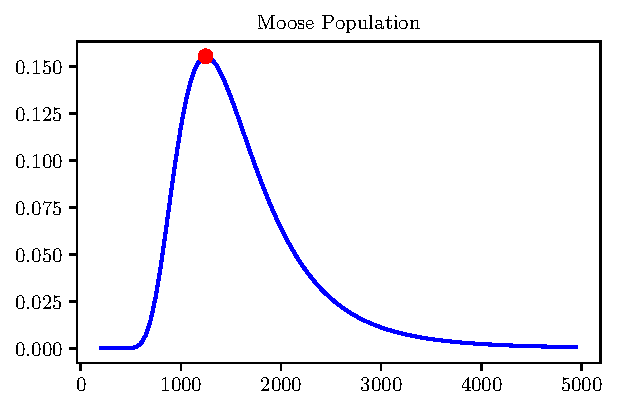
\includegraphics{img/moose.pdf}
\end{center}


\begin{python}
# using the product() function previously defined
def moosePopulation(N):
    c = 1192725059258223539848800000.0
    return c * product(N-200,N-241)/product(N-49,N)

for N in xrange(1242, 1261):
    v = moosePopulation(N)
    print "N=%d, h(N,50,200,8) = %.20f" % (N,v)
\end{python}

\N{Example}
Suppose that in a bushel of 550 apples there are 2\% rotten ones. What
is the probability that a random sample of 25 apples contains two
rotten apples? Hint: Hypergeometric distribution.

\N*{Solution:}
So, we have $N=550$ apples, of which $k=11$ are rotten. So we pick a
sample $n=25$. What's the probability $x=2$ are rotten? It's given by
\begin{equation}
\Pr(\mbox{2 rotten})=\frac{\binom{11}{2}\binom{539}{23}}{\binom{550}{25}}
\end{equation}
We can compute this by hand, finding
\begin{equation}
\begin{split}
\Pr(\mbox{2 rotten})
&=\frac{599494391824595575}{8092091399320955412}\\
&\approx 0.074083986
\end{split}
\end{equation}
so the probability is roughly $7.4\%$.

\section[Partial Summation]{Partial Summation: A Useful Tool}
\N{Definition}
Let $x\in\RR$ be any real number. We define $\intPart{x}$ to be the
greatest integer smaller than $x$. So observe
\begin{subequations}
\begin{align}
\intPart{3.1} &= 3\\
\intPart{\pi} &= 3\\
\intPart{-\E} &=-3
\end{align}
\end{subequations}
We always will have
\begin{equation}
\intPart{x}\leq x.
\end{equation}
We now may define
\begin{equation}
\fracPart{x}=x-\intPart{x}=\mbox{fractional part of $x$}
\end{equation}
and observe $0\leq\fracPart{x}<1$.

\begin{lemma}
Suppose we have a sequence $\{c_{n}\}^{\infty}_{n=1}$ and for $x\geq1$
we define a function
\begin{equation}
C(x) = \sum_{n\leq x}c_n,\quad\mbox{and}\quad C(0)=0.
\end{equation}
Let $f$ be a $C^{1}$ function, then
\begin{equation}
\sum_{n\leq x}c_{n}f(n) = C(x)f(x)-\int^{x}_{1}C(t)f'(t)\,\D t.
\end{equation}
\end{lemma}
\begin{proof}
This is a two-step proof. Step one notes
\begin{subequations}
\begin{equation}
\sum_{n\leq x}C(n)\bigl(f(n+1)-f(n)\bigr) =
C(x)f(\intPart{x})-\sum_{n\leq x}c_{n}f(n)
\end{equation}
but the left hand side is precisely
\begin{equation}
\sum_{n\leq x}C(n)\bigl(f(n+1)-f(n)\bigr) =
\int^{\intPart{x}}_{1}C(t)f'(t)\,\D t.
\end{equation}
Thus we obtain
\begin{equation}\label{eq:pf:partialSum:stepOne}
\int^{\intPart{x}}_{1}C(t)f'(t)\,\D t=C(x)f(\intPart{x})-\sum_{n\leq x}c_{n}f(n).
\end{equation}
\end{subequations}
That concludes the first step.

The second step notes
\begin{equation}\label{eq:pf:partialSum:stepTwo}
\int^{x}_{\intPart{x}}C(t)f'(t)\,\D t=C(x)f(x)-C(x)f(\intPart{x}).
\end{equation}
This uncontroversial statement should be seen immediately by the
fundamental theorem of calculus.

We then add Eq \eqref{eq:pf:partialSum:stepOne} to Eq \eqref{eq:pf:partialSum:stepTwo}
to find
\begin{subequations}
\begin{multline}
\int^{x}_{\intPart{x}}C(t)f'(t)\,\D t
+\int^{\intPart{x}}_{1}C(t)f'(t)\,\D t\\
=C(x)f(x)-C(x)f(\intPart{x})+C(x)f(\intPart{x})-\sum_{n\leq x}c_{n}f(n)
\end{multline}
which simplifies to
\begin{equation}
\int^{x}_{1}C(t)f'(t)\,\D t=C(x)f(x)+\sum_{n\leq x}c_{n}f(n)
\end{equation}
\end{subequations}
precisely as desired.
\end{proof}


\N{Example (Harmonic Series)}
We will apply our lemma to the harmonic series. How? Well, consider
\begin{equation}
H_{x}=\sum_{n\leq x}\frac{1}{n}
\end{equation}
which we consider the sequence $c_{n}=1$ and $f(t)=1/t$. Then note
\begin{equation}
C(x)=\sum_{n\leq x}1=\intPart{x}.
\end{equation}
Thus our lemma implies
\begin{equation}
H_{x} = \frac{\intPart{x}}{x}+\int^{x}_{1}\frac{\intPart{t}}{t^{2}}\,\D
t.
\end{equation}
We will try to simplify this.

First we should note that $x=\intPart{x}+\fracPart{x}$. Thus
\begin{subequations}
\begin{align}
H_{x}&=\frac{x-\fracPart{x}}{x}+\int^{x}_{1}\frac{t-\fracPart{t}}{t^{2}}\D
t\\
&=\ln(x)+\left(1-\frac{\fracPart{x}}{x}\right)-\int^{x}_{1}\frac{\fracPart{t}}{t^{2}}\D t\\
&=\ln(x)+\left(1-\int^{\infty}_{1}\frac{\fracPart{t}}{t^{2}}\D t\right)
+\int^{\infty}_{x}\frac{\fracPart{t}}{t^{2}}\D t-\frac{\fracPart{x}}{x}
\end{align}
\end{subequations}
Let
\begin{equation}
\gamma=1-\int^{\infty}_{1}\frac{\fracPart{t}}{t^{2}}\D t
\end{equation}
then our expression simplifies to
\begin{equation}
H_{x} = \ln(x)+\gamma+\int^{\infty}_{x}\frac{\fracPart{t}}{t^{2}}\D
t-\frac{\fracPart{x}}{x}.
\end{equation}
Wonderful.

But does the integral term converge? We see
\begin{subequations}
\begin{align}
\left|\int^{\infty}_{x}\frac{\fracPart{t}}{t^{2}}\D t\right|
&\leq\int^{\infty}_{x}\frac{|\fracPart{t}|}{t^{2}}\D t\\
&\leq\int^{\infty}_{x}\frac{1}{t^{2}}\D t = \frac{1}{x}.
\end{align}
\end{subequations}
Moreover this implies
\begin{equation}
\int^{\infty}_{x}\frac{\fracPart{t}}{t^{2}}\D
t-\frac{\fracPart{x}}{x}=\bigO(x^{-1}).
\end{equation}
So the expression for $H_{x}$ becomes
\begin{equation}
H_{x}=\ln(x)+\gamma+\bigO(x^{-1})
\end{equation}
but \emph{can we do better?}

\M
Lets try to figure out the next terms to order $\bigO(x^{-2})$. We will
consider
\begin{equation}
\int^{\infty}_{x}\frac{\fracPart{t}}{t^{2}}\D t-\frac{\fracPart{x}}{x}
=\int^{\infty}_{x}\frac{\fracPart{t}-\frac{1}{2}}{t^{2}}\D
t+\frac{1}{2}\int^{\infty}_{x}\frac{\D t}{t^{2}}-\frac{\fracPart{x}}{x}
\end{equation}
which simplifies to
\begin{equation}
\int^{\infty}_{x}\frac{\fracPart{t}}{t^{2}}\D t-\frac{\fracPart{x}}{x}
=\int^{\infty}_{x}\frac{\fracPart{t}-\frac{1}{2}}{t^{2}}\D t
+\frac{1}{2x}-\frac{\fracPart{x}}{x}.
\end{equation}
Now we make a claim!

\N*{Claim} The integral $\displaystyle{\int^{\infty}_{x}\frac{\fracPart{t}-\frac{1}{2}}{t^{2}}\D t=\bigO(1/x^{2})}$.

\begin{proof}
We will integrate by parts, using
\begin{equation}
u=\frac{1}{t^{2}},\quad\mbox{and}\quad\D u=\frac{-2}{t^{3}}\D t
\end{equation}
and
\begin{equation}
\D v =\left(\frac{1}{2}-\fracPart{t}\right)\D t,\quad\mbox{and}\quad
v = \int^{t}_{1}\left(\frac{1}{2}-\fracPart{u}\right)\D u.
\end{equation}
Thus the integral becomes
\begin{multline}
\lim_{R\to\infty}\int^{R}_{x}\frac{\fracPart{t}-\frac{1}{2}}{t^{2}}\D t\\
=\left.\frac{1}{t^{2}}\int^{t}_{1}\left(\frac{1}{2}-\fracPart{u}\right)\D u\right|^{t=R}_{t=x}
+2\int^{R}_{x}\frac{1}{t^{3}}\int^{t}_{1}\left(\frac{1}{2}-\fracPart{u}\right)\D u
\end{multline}
We claim that
\begin{equation}
\begin{split}
v &= \int^{[t]}_{1}
\left(\frac{1}{2}-\fracPart{u}\right)\D u
+\int^{t}_{[t]}
\left(\frac{1}{2}-\fracPart{u}\right)\D u\\
&=0+\int^{t}_{[t]}
\left(\frac{1}{2}-\fracPart{u}\right)\D u
\end{split}
\end{equation}
How can we see this? Well, we should note for any integer $k$ that
\begin{equation}
\int^{k+1}_{k}\left(\frac{1}{2}-\fracPart{u}\right)\D u=0,
\end{equation}
since it's a sawtooth function. Thus
\begin{equation}
v\leq\int^{1}_{1/2}\left(\frac{1}{2}-\fracPart{u}\right)\D
u=\frac{1}{4}.
\end{equation}
Our integral becomes
\begin{equation}
\begin{split}
\lim_{R\to\infty}\int^{R}_{x}\frac{\fracPart{t}-\frac{1}{2}}{t^{2}}\D t
&=\lim_{R\to\infty}\left.\frac{1}{t^{2}}\frac{1}{4}\right|^{t=R}_{t=x}
+2\int^{R}_{x}\frac{1}{t^{3}}\frac{1}{4}\D t\\
&\sim\bigO(x^{-2}).
\end{split}
\end{equation}
This proves the claim.
\end{proof}
Moreover, for any integer $n$, we see
\begin{equation}
\sum^{N}_{n=1}\frac{1}{n} = \ln(N)+\gamma+\frac{1}{2N}+\bigO(N^{-2}).
\end{equation}
This turns out to be a good \emph{asymptotic} approximation for harmonic
numbers. 


\chapter{Random Variables}
\M
In an election, 50 people vote. We describe all the outcomes in a sample
space $\sampleSpace$, but don't we have a valid question ``How many
voted `yes'?''? 

How can we answer such a question? \emph{Count the number of `yes'-es!}
This is done with a map
\begin{equation}
Y\colon\sampleSpace\to\NN_{0}.
\end{equation}
But what is this mapping? The number of `yes'-es, which depends on the
event. It's a \emph{random variable!}

Note that we can extend the codomain from $\NN_0$ to $\ZZ$, $\QQ$, or
$\RR$. For the sake of generality\footnote{We can sometimes include
$+\infty$, or $-\infty$, if necessary.}, we will consider $\RR$.

\N{Definition}
Let $(\sampleSpace,\mathcal{F},\Pr)$ be a probability space. We define a
\define{Random Variable} to be a function $W\colon\sampleSpace\to\RR$
such that for each $x\in\RR$ we have the set
\begin{equation}
X = \{ \omega\in\sampleSpace : W(\omega)\leq x\}
\end{equation}
be an element of $\mathcal{F}$, or in symbols $X\in\mathcal{F}$. 

\begin{rmk}
We will consider the simpler case of \define{Discrete Random Variables}
$X\colon\sampleSpace\to\ZZ$. 
\end{rmk}

The really critical theoretic property for random variables $X$ is for
any interval $B\subset\RR$, we have a set of outcomes
\begin{equation}
\{\omega\in\sampleSpace : X(\omega)\in B\}
\end{equation}
(denoted $X\in B$) which lives in the $\sigma$-algebra. Studying
$\Pr(X\in B)$ will become increasingly relevant.

\N{Examples}
Lets give a grocery list of examples.
\begin{enumerate}
\item Toss a coin $N$ times, let $H$ be the number of heads.
\item Choose a random point on $\RR^{n}$, let $D$ be the distance from
the point to the origin.
\item Take a random person from a class, let $X$ be the student's
height.
\item Let $W$ be the value of the DOW stock index at closing.
\end{enumerate}

\M
A discrete random variable has countably many values $\{x_{i}\in\RR :
i\in I\subset\ZZ\}$. We take the
convention that its codomain is a subdomain of $\ZZ$. Let $X$ be a
discrete random variable, then its \define{Probability Mass Function}
$p(x_{i}):=\Pr(X=x_{i})$.

\N{Proposition}
A probability mass function $p$ satisfies:
\begin{enumerate}
\item For any $i$, $p(x_{i})>0$
\item For any interval $B$, $\Pr(X\in B)=\sum_{x_{i}\in B}p(x_{i})$
\item We have $\sum_{i}p(x_{i})=1$.
\end{enumerate}

\N{Example}
Let $X$ be the number of heads in 2 fair coin tosses. What is its
probability mass function?

\N*{Solution:} We see there are three outcomes: 0, 1, 2. We also see
that $\Pr(X=0)=1/4$ and $\Pr(X=2)=1/4$. Thus $\Pr(X=1)=1/2$. This gives
us the probability mass function.

\N{Example}
An urn contains 20 slips of paper numbered 1, \dots, 20. We select 5 at
random, without replacement. Let $X$ be the random variable describing
the greatest value of the 5 slips selected. 

(a) Determine the probability mass function for $X$.

(b) What's the probability at least one of the slips selected is 15 or
greater?

\N*{Solution}
Well, $X$ takes the values 5, \dots, 20. There are $\binom{20}{5}$
different outcomes. So we see
\begin{equation}
\Pr(X\leq k)=\frac{\binom{k}{5}}{\binom{20}{5}}.
\end{equation}
Thus
\begin{equation}
p(k)=\Pr(X\leq k)-\Pr(X\leq k-1)
\end{equation}
and using Pascal's triangle
(theorem \ref{thm:propertiesOfBinomialCoefficients}), we have
\begin{equation}
\begin{split}
p(k) &=\frac{\binom{k}{5}-\binom{k-1}{5}}{\binom{20}{5}}\\
&=\frac{\binom{k-1}{4}}{\binom{20}{5}}
\end{split}
\end{equation}
This gives us the probability mass function.

(b) The probability one of the slips is 15 or greater can be calculated
using
\begin{equation}
\Pr(X\geq15)=\sum^{20}_{k=15}p(k).
\end{equation}
Equivalently, we can calculate it as
\begin{equation}
\begin{split}
\Pr(X\geq15)&=1-\Pr(X\leq14)=\frac{715}{15504}\\
&\approx 0.046117
\end{split}
\end{equation}
or less than a $1/20$ probability.

\N{Definition}
Let $X$ be a discrete random variable taking values $x_{1}$, $x_{2}$, \dots. 
Then the \define{Expected Value} (also called the \emph{average} or 
\emph{mean} or \emph{expectation}) for $X$ is
\begin{equation}
\expected[X] = \sum_{i}x_{i}\Pr(X=x_{i}).
\end{equation}
We also have, for any function $g\colon\RR\to\RR$,
\begin{equation}
\expected[g]=\sum_{i}g(x_{i})\Pr(X=x_{i}).
\end{equation}

\N{Example}
Let $X$ be a random variable such that $\Pr(X=1)=0.2$, $\Pr(X=2)=0.3$ and $\Pr(X=3)=0.5$. What's the expected value of $X$?

\N*{Solution:}
We find, using our definition,
\begin{equation}
\expected[X]=1\Pr(X=1)+2\Pr(X=2)+3\Pr(X=3)
\end{equation}
and this becomes
\begin{equation}
\begin{split}
\expected[X]&=1\cdot0.2+2\cdot0.3+3\cdot0.5\\
&=0.2+0.6+1.5=2.3.
\end{split}
\end{equation}
That concludes our example.

\M\label{defn:variance}
Given some discrete random variable $X$ and its expected value 
$\mu=\expected[X]$, how can we measure the ``spread'' of (the probability 
mass function for) $X$? The na\"{\i}ve solution would use $\expected|X-\mu|$, 
but this is bad since we should avoid absolute values.

So we define the \define{Variance} of $X$ as
\begin{equation}
\Var(X)=\expected(X-\mu)^{2}.
\end{equation}
Notice this intuitively measures the sum of the ``distance squared'' of the 
values $x_i$ from the expected value $\mu$. This has the ``wrong units'' 
(distance squared as opposed to distance). So we just take the square root,
and we obtain the \define{Standard Deviation}
\begin{equation}
\sigma(X)=\sqrt{\Var(X)}=\sqrt{\expected(X-\mu)^{2}}.
\end{equation}

\N{Proposition}
The expected value is linear, i.e., given random variables $X$ and $Y$ and any coefficients $c_1$, $c_2$ we have
\begin{equation}
\expected[c_1 X+c_2Y]=c_1\expected[X]+c_2\expected[Y].
\end{equation}

\M
Also note that
\begin{subequations}
\begin{align}
\Var(X) &= \expected[(X-\mu)^{2}]\\
&= \expected[X^{2}-2\mu X+\mu^{2}]\\
&=\expected[X^{2}]-2\mu\expected[X]+\mu^{2}\\
&=\expected[X^{2}]-2\mu^{2}+\mu^{2}=\expected[X^{2}]-(\expected[X])^{2}.
\end{align}
\end{subequations}
This gives us another intuition for variance!

\M
A \define{Uniform Discrete Random Variable} is a random variable taking values 
$x_1$, $x_2$, \dots, $x_n$ each with equal probability $1/n$. Such a random 
variable simply takes a random choice among $n$ numbers. Note that
\begin{subequations}
\begin{equation}
\expected[X] = \frac{x_{1}+\dots+x_{n}}{n}
\end{equation}
and
\begin{equation}
\Var[X] = \frac{x^{2}_{1}+\dots+x_{n}^{2}}{n}
-\left(\frac{x_{1}+\dots+x_{n}}{n}\right)^{2}.
\end{equation}
\end{subequations}

\N{Example}
Let $X$ be the number shown on a rolled fair die. What's $\expected[X]$ and $\Var(X)$?

\N*{Solution:}
We find
\begin{equation}
\begin{split}
\expected[X] &= \frac{1+2+\dots+6}{6}\\
&=\frac{1}{6}\left(\frac{6(7)}{2}\right)=\frac{7}{2},
\end{split}
\end{equation}
and
\begin{equation}
\expected[X^{2}]=\frac{1+2^{2}+\dots+6^{2}}{6}=\frac{91}{6}
\end{equation}
which then implies
\begin{equation}
\begin{split}
\Var(X)&=\frac{91}{6}-\left(\frac{7}{2}\right)^{2}\\
&=\frac{91}{6}-\frac{49}{4}=\frac{70}{24}=\frac{35}{12}
\end{split}
\end{equation}

\subsection{Bernoull Random Variable}
\M
Let $A$ be an event with probability $p=\Pr(A)$.
We have an \define{Indicator Function} for $A$ be a function defined as
\begin{equation}
I_{A}(x) = \begin{cases}1 & \mbox{if }x\in A\\
0 & \mbox{otherwise}\end{cases}
\end{equation}
Note $I_A$ is a random variable, since it's a function from $\sampleSpace\to\RR$.

\N*{Claim:}
$\expected[I_{A}]=p$. Really? Well, observe
\begin{equation}
\begin{split}
\expected[I_A] &= I_A(A)\Pr(A)+I_A(\comp{A})\Pr(\comp{A})\\
&= 1\cdot p + 0\cdot(1-p) = p.
\end{split}
\end{equation}
What is its variance? We see
\begin{equation}
\expected[I_{A}^{2}]=1^{2}\Pr(A)+0^{2}\Pr(\comp{A})=p,
\end{equation}
thus
\begin{equation}
\Var(I_A)=p-p^{2}=p(1-p).
\end{equation}

\M
Now, recall the ``inclusion-exclusion'' property for probability suggests
\begin{equation}
\Pr(A\cup B)=\Pr(A)+\Pr(B)-\Pr(A\cap B)
\end{equation}
which can be derived using expectation values of Bernoulli random variables. 
Recall
\begin{equation}
I_{A}+I_{\comp{A}}=1
\end{equation}
where we abuse notation and write $1$ for the constant function $I_\sampleSpace$. 
Now, we also see
\begin{equation}
I_{A\cap B}(x)=\begin{cases}1 & \mbox{if }x\in A\mbox{ and }x\in B\\
0 & \mbox{otherwise}
\end{cases}
\end{equation}
thus
\begin{equation}
I_{A\cap B}=I_{A}I_{B}.
\end{equation}
Great.

We now want to consider $I_{A\cup B}$ in terms of $I_{A}$, $I_{B}$, 
and $I_{A\cap B}$. Observe
\begin{equation}
I_{A\cup B} = 1-I_{\comp{(A\cup B)}}=1-I_{\comp{A}\cap\comp{B}}
\end{equation}
replacing $I_{\comp{A}\cap\comp{B}}$ with the product of indicator functions
gives us
\begin{equation}
I_{A\cup B}=1-I_{\comp{A}}I_{\comp{B}}.
\end{equation}
Using the fact $I_{\comp{A}}=1-I_{A}$, we have
\begin{equation}
I_{A\cup B}=1-(1-I_{A})(1-I_{B}).
\end{equation}
Using basic algebra, expanding out the right hand side, we find
\begin{equation}
I_{A\cup B}=I_{A}+I_{B}-I_{A\cap B}.
\end{equation}
Now, we take expectation values to find
\begin{equation}
\begin{split}
\Pr(A\cup B) &=\expected(I_{A\cup B}) 
= \expected[I_A]+\expected[I_B]-\expected[I_{A\cap B}]\\
&=\Pr(A)+\Pr(B)-\Pr(A\cap B).
\end{split}
\end{equation}
This gives us an alternate proof of the inclusion-exclusion principle.

\N{Hat Checker Problem Redux}
We can use indicator functions to solve the hat checker problem, which we 
introduced in subsection \ref{subsec:hatCheckProblem}. Let $\pi$ be a 
permutation of $n$ elements, we want to find the number of fixed points. Let
\begin{equation}
X(\sigma)=\mbox{number of fixed points of $\sigma$}.
\end{equation}
We introduce the indicator function
\begin{equation}
I_{i}(\pi) = \begin{cases}
1 & \mbox{if $i$ is a fixed point of $\pi$}\\
0 & \mbox{otherwise}
\end{cases}
\end{equation}
We now fix a number $r$ such that $0\leq r\leq n-2$. Why $n-2$? We want to
sum over the permutations which do not fix all the points. If we fix $n-1$ points,
then we fix all the points (think about it: if we give $n-1$ people their hats 
correctly, the remaining hat must belong to the remaining person!). 

So we now set
\begin{equation}
\mathcal{S}_{r}=\sum_{\pi\in S_{n}}I_{j_1}(\dots)I_{j_r}(1-I_{k_{r+1}})%
(\dots)(1-I_{k_{n}})
\end{equation}
where we sum over all permutations. Observe there are $n!$ terms in the sum.

If $X(\sigma)\neq r$, we claim $\mathcal{S}_{r}=0$. Why? Well, if 
$X(\sigma)>r$, then one of the $(1-I_{k_{\textstyle{*}}})$ factors vanishes
in every term. If $X(\sigma)<r$, then one of the $I_{j_{\normalsize *}}$ factors
vanishes in every term. 

How many different scenarios do we have $X(\sigma)=r$? There are $r!$
different ways to have fixed points, and $(n-r)!$ different ways to permute
the non-fixed points. Thus
\begin{equation}
\mathcal{S}_{r}=r!(n-r)!
\end{equation}
as desired. So
\begin{equation}
\mathcal{S}_{r}(\sigma) = \begin{cases}r!(n-r)! & \mbox{if $X(\sigma)=r$}\\
0 & \mbox{otherwise}\end{cases}
\end{equation}
Thus we can construct an indicator function
\begin{equation}
\mathcal{I}_{r}=\frac{\mathcal{S}_{r}}{r!(n-r)!}
\end{equation}
which tells us if a permutation has $r$ fixed points.

\N*{Puzzle:}
What's $\expected[\mathcal{I}_{r}]$?

\medbreak
Using linearity, we have
\begin{equation}
\expected[\mathcal{I}_r]=\frac{1}{r!(n-r)!}\expected[\mathcal{S}_{r}],
\end{equation}
and we need to compute $\expected[\mathcal{S}_{r}]$. We find
\begin{equation}
\expected[\mathcal{S}_r] = \expected\left(\sum_{\pi}I_{j_1}(\dots)I_{j_r}(1-I_{k_{r+1}})(\dots)(1-I_{k_n})\right)
\end{equation}
then we expand the $(1-I_{k_{\textstyle *}})$ factors
\begin{multline}
\expected[\mathcal{S}_r] = \expected\Bigg(\sum_{\pi}I_{j_1}(\dots)I_{j_r}
\times\biggl[1-(I_{k_{r+1}}I_{k_{r+2}}+\dots+I_{k_{n-1}}I_{k_n}) \\
+(\dots)+(-1)^{n-r}I_{k_{r+1}}(\dots)I_{k_n}\biggr]\Bigg)
\end{multline}
Now, we claim that
\begin{equation}
\expected[I_{j_1}(\dots)I_{j_{r}}I_{k_{r+s}}]=\expected[I_{j_1}(\dots)I_{j_{r}}I_{k_{r+1}}]
\end{equation}
for $s=1,\dots,n-r$. This means our sum becomes
\begin{equation}
\expected[\mathcal{S}_r]=\sum_{\pi}\sum^{n-r}_{s=0}(-1)^{s}\binom{n-r}{s}
\expected[I_{j_1}(\dots)I_{j_r}I_{k_{r+1}}(\dots)I_{k_{r+s}}]
\end{equation}
where $0\leq s\leq n-r$. So we see
\begin{equation}
\expected[I_{j_1}(\dots)I_{j_r}I_{k_{r+1}}(\dots)I_{k_{r+s}}]=\frac{(n-r-s)!}{n!}
\end{equation}
as there are $n!$ permutations with only $(n-r-s)!$ permutations fixing the 
given entries.

Now, we combine everything together, and find
\begin{subequations}
\begin{align}
\expected[\mathcal{I}_r] &=
\frac{1}{r!(n-r)!}\expected[\mathcal{S}_r]\\
&=\frac{1}{r!(n-r)!}\sum_{\pi}\sum^{n-r}_{s=0}(-1)^{s}\binom{n-r}{s}\frac{(n-r-s)!}{n!}\\
&=\frac{1}{r!(n-r)!}n!\sum^{n-r}_{s=0}(-1)^{s}\binom{n-r}{s}\frac{(n-r-s)!}{n!}\\
&=\frac{1}{r!}\sum^{n-r}_{s=0}\frac{(-1)^{s}}{s!}
\end{align}
\end{subequations}
So, summarizing the main conclusion, the probability that a random permutations 
has exactly $r$ fixed points is given by
\begin{equation}
\Pr(X=r)=\frac{1}{r!}\left(\frac{1}{2!}-\frac{1}{3!}+\dots+\frac{(-1)^{n-r}}{(n-r)!}\right).
\end{equation}
This holds for $0\leq r\leq n-2$. For $r=0$, this converges quickly to the value
\begin{equation}
\frac{1}{\E}=0.367 879 441 171\dots
\end{equation}
We have thus derived another solution to the hat check problem using Bernoulli 
random variables.

\subsection{Poisson Distribution}
\N{Derivation}
Consider the binomial distribution
\begin{equation}
b(n,p) = \binom{n}{k}p^{k}(1-p)^{n-k}.
\end{equation}
We take $\lambda=np$ to be the ``intensity''. Then we can re-write the
distribution as
\begin{subequations}
\begin{align}
b(n,p) &= \frac{n!}{k!(n-k)!}\left(\frac{\lambda}{n}\right)^{k}
\left(1-\frac{\lambda}{n}\right)^{n-k}\\
&=\left[\frac{n-(k-1)}{n}(\cdots)\frac{n-(k-k)}{n}\right]\frac{\lambda^{k}}{k!}\left(1-\frac{\lambda}{n}\right)^{n}\left[\left(1-\frac{\lambda}{n}\right)^{-k}\right]\\
&=\left[\left(1-\frac{(k-1)}{n}\right)(\cdots)\left(1-\frac{(k-k)}{n}\right)\right]\nonumber\\
&\phantom{=}\qquad\times\frac{\lambda^{k}}{k!}\left(1-\frac{\lambda}{n}\right)^{n}\left[\left(1-\frac{\lambda}{n}\right)^{-k}\right].
\end{align}
\end{subequations}
Now we take the limit $n\to\infty$ while fixing $k$:
\begin{align}
\lim_{n\to\infty}b(n,p)&=\lim_{n\to\infty}\left[\left(1-\frac{(k-1)}{n}\right)(\cdots)\left(1-\frac{(k-k)}{n}\right)\right]\frac{\lambda^{k}}{k!}\left(1-\frac{\lambda}{n}\right)^{n}\left[\left(1-\frac{\lambda}{n}\right)^{-k}\right]\nonumber\\
&=[1]\frac{\lambda^{k}}{k!}\E^{-\lambda}[1].
\end{align}
This gives us the \define{Poisson distribution}\index{Poisson distribution}\index{distribution!Poisson}\marginpar{Poisson distribution}
\begin{equation}
f(k,\lambda)=\frac{\lambda^{k}}{k!}\E^{-\lambda}.
\end{equation}

\begin{xca}
Consider the sample space $\sampleSpace=\NN_{0}$ obtained by the Poisson
process. Calculate $\Pr(\sampleSpace)$.
\end{xca}
\N*{Solution:}
We see that
\begin{equation}
\Pr(\sampleSpace)
= \sum_{k=0}^{\infty}\frac{\E^{-\lambda}\lambda^{k}}{k!}
\end{equation}
but we can rearrange factors, and find
\begin{equation}
\Pr(\sampleSpace)
= \E^{-\lambda}\sum^{\infty}_{k=0}\frac{\lambda^{k}}{k!}=\E^{-\lambda}\E^{\lambda}=1.
\end{equation}
Thus, in the $f(k,\lambda)$, the factor $\E^{-\lambda}$ is a
normalization constant. 

\N{Interpretation}
We interpret $\lambda$ as the number of events in some unit of time. The
parameter $k$ indicates the number of events we wonder about (i.e., we
ask ``What's the probability $k$ events will happen?''). 

\N{Example}
Airlines find that passangers who make reservations fail to appear with
probability $1/10$, independent of other passangers. Acme Airlines sell
10 tickets for their 9 seat airplane, and 20 tickets for their 18 seat
plane. Which plane is often over-booked?

\N*{Solution One:}
Lets write
\begin{equation}
f(n,k)=\binom{n}{k}\left(\frac{1}{10}\right)^{k}\left(1-\frac{1}{10}\right)^{n-k}
\end{equation}
for the probability $k$ people with reservations don't appear. We see
the probability the smaller plane is overbooked occurs only when all 10
people appear, which has probability
\begin{equation}\label{eq:probSmallPlaneOverbooked}
f(10,0)=\left(\frac{9}{10}\right)^{10}=0.3486784401.
\end{equation}
The larger plane is overbooked when 19 or 20 people appear, which occurs
with probability
\begin{equation}\label{eq:probBigPlaneOverbooked}
\begin{split}
f(20,0)+f(20,1)
&=20\frac{1}{10}\left(\frac{9}{10}\right)^{19}+\left(\frac{9}{10}\right)^{20}\\
&=0.39174699812516770581.
\end{split}
\end{equation}
We see the larger plane gets overbooked a tad more often than the
smaller plane.

\N*{Solution Two:}
Using the Poisson distribution, we will count the number of passangers
that are absent as the ``intensity''. So
$\lambda_{s}=n\cdot1/10$ or $\lambda_{s}=1$. We see
\begin{equation}
\mathrm{Poi}(k,\lambda_{s})=\frac{\E^{-1}}{k!}
\end{equation}
and we get overbooked for
\begin{equation}
\mathrm{Poi}(0,\lambda_{s})=\E^{-1}\approx 0.36787944
\end{equation}
which is within 2\% of Eq \eqref{eq:probSmallPlaneOverbooked}.

But for the larger plane, we see $\lambda_{l}=2$ is the intensity of
absent people, so
\begin{subequations}
\begin{equation}
\mathrm{Poi}(0,\lambda_{l})=\E^{-2}
\end{equation}
and
\begin{equation}
\mathrm{Poi}(1,\lambda_{l})=2\E^{-2}
\end{equation}
thus
\begin{equation}
\mathrm{Poi}(19,\lambda_{l})+
\mathrm{Poi}(20,\lambda_{l})=3\E^{-2}\approx 0.4060058
\end{equation}
\end{subequations}
which is within $1.5\%$ of Eq \eqref{eq:probBigPlaneOverbooked}.
We see these approximations are quite good!

\section{Expected Values}
\M
If we have a discrete random variable $X\colon\sampleSpace\to\RR$, we
can ask what's its \emph{expected value}? What does this mean? We mean,
if $X=x_{j}$ for $j\in\NN$, we want to consider the expression
\begin{equation}
\expected[X]=\sum_{j\in\NN}x_{j}\Pr(X=x_{j}).
\end{equation}
The intuition is that
\begin{equation}
\expected[X] = \frac{1}{N(\sampleSpace)}\sum_{j\in\NN}x_{j}N(x_{j})
\end{equation}
which is precisely what we have.

\N{Example}
Recall Example \ref{ex:studentGuessingOnExam} when a student guesses on
a true-false exam. What's the expected value of a student guessing on a
10 question true-false exam?

\N*{Solution:}
We see that
\begin{equation}
\expected[X] = \sum^{10}_{n=0}n\cdot\binom{10}{n}2^{-10}
\end{equation}
We recall
\begin{equation}
(1+x)^{n}=\sum^{n}_{k=0}\binom{n}{k}x^{k}
\end{equation}
thus taking its derivative gives us
\begin{equation}
n(1+x)^{n-1}=\sum^{n}_{k=0}k\binom{n}{k}x^{k-1}.
\end{equation}
We set $x=1$ and obtain
\begin{equation}
n2^{n-1}=\sum^{n}_{k=0}k\binom{n}{k}.
\end{equation}
We thus deduce
\begin{equation}
\expected[X]=2^{-10}\cdot 10\cdot2^{9}=5.
\end{equation}
An anticlimactic solution: guessing should give a score of 50\%.

\begin{thm}
The expectation operator satisfies the following properties:
\begin{enumerate}
\item If $X\geq0$, then $\expected[X]\geq0$
\item For any $a,b\in\RR$ we have
$\expected[aX+bY]=a\expected[X]+b\expected[Y]$
\item The random variable ${\bf 1}$ which takes the constant value $1$
satisfies $\expected[{\bf 1}]=1$.
\end{enumerate}
\end{thm}
\begin{proof}
(1) We see that if $X$ takes values $x_j\geq0$, then $\Pr(X=x_j)\geq0$,
and the product of two positive real numbers is positive. The sum of
positive real numbers is itself a positive real number.

(2) Linearity follows immediately:
\begin{subequations}
\begin{align}
\expected[aX+bY] &=\sum_{\omega}a\omega\Pr(X=\omega)+b\omega\Pr(Y=\omega)\\
&= \sum_{x}ax\Pr(X=x) + \sum_{y}by\Pr(Y=y)\\
&=a\sum_x x\Pr(X=x)+b\sum_y y\Pr(Y=y) = a\expected[X]+b\expected[Y].
\end{align}
\end{subequations}

(3) Obvious, since it becomes a sum of probabilities which must be unity.
\end{proof}

\subsection{Joint Distributions}
\N{Definition}
Let $X$, $Y$ be discrete random variables. Their \define{Joint
Distribution} $F\colon\RR^{2}\to[0,1]$ is given by
\begin{equation}
F(x,y)=\Pr(X\leq x, Y\leq y)
\end{equation}
and their \define{Joint Mass Function} is
\begin{equation}
f(x,y) = \Pr(X=x,Y=y).
\end{equation}
We sometimes use the notation $f_{X,Y}(x,y)$ to make it clear what the
random variables are.
\N{Definition}
We see that $X$ and $Y$ are \define{Independent} if and only if
\begin{subequations}
\begin{align}
f_{X,Y}(x,y)
&= \Pr(X=x,Y=y)\\
&=\Pr(X=x)\Pr(Y=y)\\
&=f_{X}(x)f_{Y}(y)
\end{align}
\end{subequations}
Note we induce this notion using the usual notion of independence.

\N{Definition}
We have the \define{Covariance} of $X$ and $Y$ be
\begin{equation}
\cov(X,Y)=\expected[XY]-\expected[X]\expected[Y]
\end{equation}
and the \define{Correlation Coefficient}
\begin{equation}
\rho(X,Y)=\frac{\cov(X,Y)}{\sqrt{\Var(X)\Var(Y)}}
\end{equation}
Recall we defined the variance $\Var(X)$ in \Mref{defn:variance}.

\begin{lemma}[Independence Condition]
Let $X$, $Y$ be random variables. They are independent if and only if 
\begin{equation}
\cov(X,Y)=0.
\end{equation}
\end{lemma}
\begin{proof}
We see that
\begin{equation}
\begin{split}
\expected[XY]-\expected[X]\expected[Y]
&=\sum_{x,y}xy\Pr(X=x,Y=y)-x\Pr(X=x)y\Pr(Y=y)\\
&=\sum_{x,y}xy\bigl(\Pr(X=x,Y=y)-\Pr(X=x)\Pr(Y=y)\bigr)
\end{split}
\end{equation}
but we see independence for joint distributions precisely occurs when
\begin{equation}
\bigl(\Pr(X=x,Y=y)-\Pr(X=x)\Pr(Y=y)\bigr)=0
\end{equation}
for any $x$ and $y$.
\end{proof}

\begin{thm}[Cauchy-Schwarz Inequality]
Let $X$, $Y$ be random variables. Then
\begin{equation}
\bigl(\expected[XY]\bigr)^{2}\leq\expected[X^{2}]\expected[Y^{2}]
\end{equation}
with equality if and only if $\Pr(aX=bY)=1$ for some $a,b\in\RR$ (at
least one of which is nonzero).
\end{thm}
\begin{proof}
We introduce a new random variable
\begin{equation}
Z = aX + bY
\end{equation}
where $a,b\in\RR$. Suppose $a\geq0$. Then
\begin{equation}
0\leq\expected[Z^{2}]=a^{2}\expected[X^{2}]+b^{2}\expected[Y^{2}]-2ab\expected{XY}.
\end{equation}
We consider the right hand side as a quadratic function in $a$. When
does it have a real root? When
\begin{subequations}\label{eq:Cauchy-Schwarz:prob:proof}
\begin{equation}
B^{2}-4AC\leq0
\end{equation}
or for us
\begin{equation}
4b^{2}\expected[XY]^{2}-4\expected[X^{2}]\cdot
b^{2}\expected[Y^{2}]\leq0
\end{equation}
\end{subequations}
For nonzero $b$, we have the desired result immediately.

Observe one real root of Eq \eqref{eq:Cauchy-Schwarz:prob:proof}
implies
\begin{subequations}
\begin{equation}
\expected[Z^{2}]=0
\end{equation}
which implies
\begin{equation}
Z=0\quad\mbox{with probability }1.
\end{equation}
Thus
\begin{equation}
aX-bY=0
\end{equation}
\end{subequations}
with probability 1.
\end{proof}

\subsection{Conditional Distributions and Expectations}

Let $X$ and $Y$ be two discrete random variables on
$(\sampleSpace, \mathcal{F}, \Pr)$.

\begin{defn}
The \define{Conditional Distribution Function} of $Y$ given $X=x$,
written $F_{Y|X}(-|x)$, is defined by
\begin{equation}
F_{Y|X}(y|x) = \Pr(y\leq Y|X=x)
\end{equation}
for any $x$ such that $\Pr(X=x)>0$.

The \define{Conditional Probability Function} (or ``\emph{Conditional
Mass Function\/}'') of $Y$ given $X=x$, written $f_{Y|X}(-|x)$, is
defined as
\begin{equation}
f_{Y|X}(y|x)=\Pr(Y=y|X=x)
\end{equation}
\end{defn}
\begin{rmk}
Note this definition implies
\begin{equation}
f_{Y|X}=\frac{f_{Y,X}}{f_{X}}
\end{equation}
and that $X$ and $Y$ are independent if and only if
\begin{equation}
f_{Y|X}=f_{Y}.
\end{equation}
This justifies the choice of notation.
\end{rmk}
\begin{rmk}
Given $X=x$, we may ``define''
\begin{equation}\label{eq:defn:rmk:condExpect}
\begin{split}
\expected[Y|X=x] &\eqdef \sum_{y}yf_{Y|X}(y|x)\\
&=\mbox{conditional expectation of $Y$ given $(X=x)$}
\end{split}
\end{equation}
We may think of this as a function of $x$:
\begin{equation}
\psi(x) = \expected[Y|X=x].
\end{equation}
Thus the expected value may be thought of as a function of $X$:
\begin{equation}
\psi(X) = \expected[Y|X].
\end{equation}
This is a mildly sloppy abuse of notation.
\end{rmk}
\begin{defn}
Let $\psi(x)=\expected[Y|X=x]$. Then the \define{Conditional
Expectation} of $Y$ given $X$ written $\expected[Y|X]$ is precisely
$\psi(X)$. Note that $\expected[Y|X]$ is a random variable. 
\end{defn}

\begin{thm}
Given random variables $X$, $Y$ as specified, then
\begin{equation}
\expected\bigl[\expected[Y|X]\bigr] = \expected[Y].
\end{equation}
\end{thm}
\begin{proof}
This is a classic ``follow-your-nose and unravel the definitions'' type proof.
\begin{subequations}
\begin{align}
\expected\bigl[\expected[Y|X]\bigr]
&=\sum_{x}f_{X}(x)\left(\sum_{y}yf_{Y|X}(y|x)\right)\\
&=\sum_{y}y\sum_{x}f_{X,Y}(x,y)\\
&=\sum_{y}yf_{Y}(y)=\expected[Y].
\end{align}
\end{subequations}
We just began with Eq \eqref{eq:defn:rmk:condExpect} and ``followed our nose''!
\end{proof}

Note more generally, we have
\begin{equation}
\expected\bigl[\expected[Y|X]g(X)\bigr]=\expected[Yg(X)].
\end{equation}
The proof is simple:
\begin{subequations}
\begin{align}
\expected\bigl[\psi(x)g(x)\bigr]
&=\sum_{x}\psi(x)g(x)\Pr(X=x)\\
&=\sum_{y}y\sum_{x}\Pr(Y=y|X=x)g(x)\Pr(X=x)\\
&=\sum_{x,y} yg(x)\Pr(X=x,Y=y)=\expected[Yg(X)].
\end{align}
\end{subequations}
% pg 15 of notes 7
\begin{thm}
Let $a,b\in\RR$, and $X$, $Y$, $Z$ be random variables.
\begin{enumerate}
\item $\expected[aY+bZ|X]=a\expected[Y|X]+b\expected[Z|X]$
\item $\expected[Y|X]\geq0$ if $Y\geq0$
\item $\expected[1|X]=1$
\item If $X$ and $Y$ are independent, then $\expected[Y|X]=\expected[Y]$
\item $\expected[Yg(X)|X]=g(X)\expected[Y|X]$ where $g\colon\RR\to\RR$
\item $\expected\bigl[\expected[Y|X,Z]|X\bigr]=\expected[Y|X]$ and $\expected\bigl[\expected[Y|X]|X,Z\bigr]=\expected[Y|X]$.
\end{enumerate}
\end{thm}


\vfill\eject
\appendix
\chapter{Set Theory}
\N{Overview}
This section is just to establish the notation used for set theory.
We use a ``naive set theory'', which --- for the author --- is really
just ZF+GC. 

\N{Global Choice}
Recall we have quantifiers $\forall$ and $\exists$. We can also have a
quantifier $\varepsilon$ which has the form
\begin{equation}
\varepsilon x : P(x)
\end{equation}
and it returns the object $x$ which satisfies the predicate $P(x)$, if
one exists. If there is no such $x$ (e.g., $P(x)$ is a contradiction),
then it returns an arbitrary object.

This $\varepsilon$ operator is called the \define{Global Choice
Operator}. 

\N{Definition} A \define{Set} is a well-defined collection of ``stuff''
without duplicates.

\N{Definition}
If $X$ is a set, and $x$ is an object, if $x$ lives in the collection
$X$ we write $x\in X$ and call it a \define{Element} or \define{Member}
of $X$. We will write sets using capital Latin letters unless otherwise
indicates. If $y$ does not belong to $X$, we write $y\notin X$.

Note \emph{any type of object} can belong to a set. For example, we can
have a set of selected sets, the set of integers (usually denoted
$\mathbb{Z}$), etc.

\textsc{Caution}: It is illegal (``meaningless'') to write $X\in X$ or $X\notin X$. 

\N{Example} The empty collection is a set, denoted $\emptyset$ and
called the \define{Empty Set}. It is defined by the condition, for any
$x$, we have $x\notin \emptyset$.

\N{Example} 
The collection of natural numbers $\NN=\{\,1,2,3,\dots\,\}$, the natural
numbers with zero $\NN_{0}=\{\,0,1,2,3,\dots\,\}$. The integers
$\ZZ=\{\dots,-1,0,1,\dots\,\}$. These are all sets.

\N{Non-Example (Universe)}
Consider $\mathcal{U}$ the well-defined collection of all sets. It is
not a set, since it is illegal to write $\mathcal{U}\in\mathcal{U}$. No,
the universe is usually something ``bigger'' than a set (it's
a \emph{class}). We usually don't work with classes, and so we won't
worry about them. But we'd like to note the collection of all sets
$\mathcal{U}$ is called the \define{Universe}.

\N{Definition}
Let $X$ and $Y$ be sets. If every element $x\in X$ belongs to $Y$, and
every $y\in Y$ belongs to $X$, then we say the two sets are
\define{Equal} and write $X=Y$.

\N{Definition}
Let $X$ and $Y$ be sets. If every element $x\in X$ belongs to $Y$, then
we write $X\subset Y$ and call $X$ a \define{Subset} of $Y$.

\N{Theorem} We have $X=Y$ if and only if $X\subset Y$ and $Y\subset X$.

\N{Definition}
Let $Y$ be a set. A \define{Proper Subset} $X$ of $Y$ consists of a
subset that is not equal to $Y$. That is: $X\subset Y$ and $X\neq Y$. We
indicate proper subsets by writing $X\propersubset Y$.

\N{Examples} Observe we have $\NN\propersubset\NN_{0}\propersubset\ZZ$.

\N{Example} For any set $X$, we have $X\subset X$ but
$X\not\propersubset X$.

\N{Definition}
Let $X$ be any set. Then the \define{Power Set} of $X$ is the collection
$\powerset(X)$ of subsets $Y\subset X$. Note this implies
$X\in\powerset(X)$. 

\N{Proposition}
Let $X$ be any set. Then $\emptyset\in\powerset(X)$ and
$X\in\powerset(X)$.

\N{Definition}
An \define{Ordered Tuple} $(a,b)$ is a pair of mathematical objects $a$,
$b$. The first slot $a$ is the first component (sometimes called
the \emph{first coordinate}).

We write $(a,b)=(x,y)$ if and only if $a=x$ and $b=y$.

More generally, if we have $n$ objects, we can form the ordered
$n$-tuple $(x_{1},\dots,x_{n})$. Again, equality is defined
component-wise. 

\N{Definition}
Let $X$ and $Y$ be sets. Then their \define{Cartesian Product} is a set
$X\times Y$ consisting of ordered pairs $(x,y)\in X\times Y$ where $x\in
X$, $y\in Y$.

Again, we can generalize this to the Cartesian product of any number of
sets $X_1\times\dots\times X_n$ consisting of ordered $n$-tuples.

\N{Definition}
A \define{Function} $f\colon X\to Y$ associates to each $x\in X$
precisely one $y\in Y$ usually denoted $y=f(x)$. 

Sometimes mathematicians assert functions are sets. Well, a function $f$
is a subset $f\subset X\times Y$ with the property for each $x\in X$, we
have precisely one ordered pair $(x,y)\in f$.

\N{Example}
Let $X$ be any set.
The identity function $\mathrm{id}\colon X\to X$ defined by
$\mathrm{id}(x)=x$ is a function on $X$.


\begin{thebibliography}{99}\small
\bibitem{grimmetStirzaker}
Geoffrey Grimmet and David Stirzaker,\newblock
\emph{Probability and Random Processes}.\newblock
Third ed., Oxford University Press, 2006.
\bibitem{gravner}
Janko Gravner,\newblock
Lecture notes on Probability.\newblock
UC Davis Math 135A, 2011. Eprint: \href{http://www.math.ucdavis.edu/~gravner/MAT135A/resources/lecturenotes.pdf}{\nolinkurl{math.ucdavis.edu/~gravner}}
\bibitem{miller:2004}
L.E.~Miller,\newblock
``Evaluation of Network Reliability Calculation Method.''\newblock
Eprint \url{http://www.antd.nist.gov/wctg/netanal/EvalNetRel.pdf}, 2004.
\bibitem{virtualLab}
Kyle Siegrist,\newblock
``Virtual Laboratories in Probability and Statistics.''\newblock
Eprint \href{http://www.math.uah.edu/stat/index.html}{\tt math.utah.edu/stat/}, accessed November
9, 2012.
\bibitem{tomE} Tom E (\href{http://mathoverflow.net/users/3200/tom-e}{\tt mathoverflow.net/users/3200}),\newblock 
``What's the use of a complete measure?''\newblock
Eprint \href{http://mathoverflow.net/questions/11554}{\tt mathoverflow.net}, January 12, 2010.
\end{thebibliography}


\end{document}
